% !TeX program = xelatex
% !TeX encoding = UTF-8
% Spedizione P07 · Terreno, pendenze e sintesi territoriali
% Presentazione della spedizione P07 nella serie planetaria di GeoStat Lab.
% Compilazione: xelatex -interaction=nonstopmode P07_Terreno.tex (due passaggi)
% 27 slide. Diagrammi TikZ, figure vettoriali da R/P07_figure.R, codice R, dati ed esperimenti inclusi.
\RequirePackage{fix-cm}
\documentclass[12pt,aspectratio=1610]{beamer}
\geometry{paperwidth=20cm,paperheight=12.5cm}
\usepackage[italian,provide=*]{babel}
\usepackage{fontspec,adjustbox,tabularx}
\IfFontExistsTF{NimbusSans-Regular.otf}{
\setsansfont{NimbusSans-Regular.otf}[BoldFont=NimbusSans-Bold.otf,ItalicFont=NimbusSans-Italic.otf,BoldItalicFont=NimbusSans-BoldItalic.otf]
\setmainfont{NimbusSans-Regular.otf}[BoldFont=NimbusSans-Bold.otf,ItalicFont=NimbusSans-Italic.otf,BoldItalicFont=NimbusSans-BoldItalic.otf]
}{
\setsansfont{TeX Gyre Heros}
\setmainfont{TeX Gyre Heros}
}
\IfFontExistsTF{DejaVu Sans Mono}{
\setmonofont{DejaVu Sans Mono}[Scale=.88]
}{\setmonofont{Latin Modern Mono}[Scale=.88]}
\usefonttheme{professionalfonts}
\usepackage{amsmath,amssymb,booktabs,array,graphicx,tikz,bookmark}
\usetikzlibrary{calc,positioning,arrows.meta}
\graphicspath{{Figure/}}
\definecolor{Paper}{HTML}{F8F6F1}
\definecolor{Ink}{HTML}{253344}
\definecolor{Navy}{HTML}{15283E}
\definecolor{Quantum}{HTML}{5146A5}
\definecolor{Classical}{HTML}{087C74}
\definecolor{Muted}{HTML}{657180}
\definecolor{Rule}{HTML}{D6DAD9}
\definecolor{Night}{HTML}{112236}
\definecolor{Lilac}{HTML}{ABB5FF}
\definecolor{Mint}{HTML}{72D8C8}
\setbeamercolor{background canvas}{bg=Paper}
\setbeamercolor{normal text}{fg=Ink}
\setbeamertemplate{navigation symbols}{}
\setbeamertemplate{headline}{}
\setbeamertemplate{footline}{}
\setbeamersize{text margin left=0pt,text margin right=0pt}
\hypersetup{colorlinks=true,linkcolor=Classical,urlcolor=Classical,pdfpagemode=UseOutlines,pdfstartview=Fit,
 pdftitle={Spedizione P07 · Terreno, pendenze e sintesi territoriali},pdfauthor={GeoStat Lab · materiali di Marzio De Corato},
 pdfsubject={GeoStat Lab · P07}}
\bookmarksetup{open,openlevel=0,depth=2}
\newsavebox{\BodyBox}
\newsavebox{\SideBox}
\newsavebox{\RecallBox}
\newsavebox{\TitleBox}
\newcommand{\MeasureBox}[2]{\typeout{REVIEWBOX:#1:\the\wd#2:\the\ht#2:\the\dp#2}}

% Revisione completa: diagrammi TikZ, formalismo e box R.
\usepackage[most]{tcolorbox}
\usepackage{listings}
\usetikzlibrary{fit,backgrounds,matrix,decorations.pathreplacing}
\definecolor{GeoA}{HTML}{1D7890}
\definecolor{GeoB}{HTML}{C57E42}
\definecolor{GeoC}{HTML}{7363AA}
\definecolor{GeoTint}{HTML}{F0F4F3}
\lstdefinestyle{GeoR}{language=R,basicstyle=\ttfamily\fontsize{9.2}{12.2}\selectfont,
 keywordstyle=\color{Quantum}\bfseries,commentstyle=\color{Classical},stringstyle=\color{GeoB},
 numbers=left,numberstyle=\tiny\color{Muted},numbersep=4pt,showstringspaces=false,
 columns=fullflexible,keepspaces=true,breaklines=true,xleftmargin=1.15em,
 frame=none,aboveskip=0pt,belowskip=0pt,tabsize=2}
\newsavebox{\PilotLeftBox}
\newsavebox{\PilotRightBox}
\newcommand{\PLabel}[1]{\par{\color{Classical}\bfseries\fontsize{9}{11}\selectfont\MakeUppercase{#1}}\par\vspace{1.8mm}}
\newcommand{\PBody}[1]{\par{\fontsize{11.3}{14.8}\selectfont #1\par}}
\newcommand{\PSmall}[1]{\par{\fontsize{9.8}{13.1}\selectfont #1\par}}
\newcommand{\PCode}[2]{%
\begin{tcolorbox}[enhanced,arc=1.8mm,boxrule=.65pt,
  colback=white,colframe=Classical!75!Navy,colbacktitle=Navy,
  coltitle=white,fonttitle=\bfseries\fontsize{9.6}{12}\selectfont,
  title={#1},left=1.7mm,right=1.3mm,top=1.5mm,bottom=1.3mm,
  before skip=1mm,after skip=1mm]
\lstinputlisting[style=GeoR]{Codice/#2}
\end{tcolorbox}}
\newcommand{\PInfo}[1]{%
\begin{tcolorbox}[enhanced,arc=1.6mm,boxrule=.55pt,colback=GeoTint,
 colframe=Rule!80!Classical,left=2.3mm,right=2.3mm,top=2mm,bottom=2mm,
 before skip=1mm,after skip=1mm]
\PSmall{#1}\end{tcolorbox}}
\tikzset{
 pFlow/.style={draw=Classical!45,fill=white,rounded corners=2mm,
  line width=.7pt,align=center,minimum height=1.1cm,font=\sffamily\fontsize{10}{12}\selectfont},
 pEdge/.style={-{Latex[length=2.3mm]},draw=Classical,line width=.95pt},
 pGroup/.style={draw=Rule,fill=white,rounded corners=2mm,line width=.65pt},
 pDotA/.style={circle,fill=GeoA,inner sep=1.25pt},
 pDotB/.style={circle,fill=GeoB,inner sep=1.25pt},
 pDotC/.style={circle,fill=GeoC,inner sep=1.25pt}
}
\newcommand{\PilotChrome}[4]{%
  \node[anchor=north west,inner sep=0,text width=17.7cm] at ([xshift=.95cm,yshift=-.55cm]current page.north west) {\color{Navy}\bfseries\fontsize{20.6}{24.5}\selectfont #1};
  \node[anchor=north east,inner sep=0] at ([xshift=19.05cm,yshift=-.14cm]current page.north west) {\color{Classical}\fontsize{8}{10}\selectfont\hyperlink{slide2}{#2}};
  \draw[Classical,line width=1.2pt] ([xshift=.95cm,yshift=-1.7cm]current page.north west)--([xshift=2.35cm,yshift=-1.7cm]current page.north west);
  \draw[Rule,line width=.65pt] ([xshift=.95cm,yshift=-10.36cm]current page.north west)--([xshift=19.05cm,yshift=-10.36cm]current page.north west);
  \node[anchor=north west,inner sep=0] at ([xshift=.96cm,yshift=-10.55cm]current page.north west) {\color{Classical}\bfseries\fontsize{9.1}{12}\selectfont DA RICORDARE};
  \node[anchor=north west,inner sep=0,text width=14.3cm] at ([xshift=4.2cm,yshift=-10.53cm]current page.north west) {\color{Ink}\fontsize{10.3}{13.8}\selectfont #4};
  \draw[Rule,line width=.35pt] ([xshift=.95cm,yshift=-11.92cm]current page.north west)--([xshift=19.05cm,yshift=-11.92cm]current page.north west);
  \node[anchor=north west,inner sep=0] at ([xshift=.95cm,yshift=-12.06cm]current page.north west) {\color{Muted}\fontsize{7.7}{9.2}\selectfont Spedizione P07 · Terreno, pendenze e sintesi territoriali};
  \node[anchor=north east,inner sep=0] at ([xshift=19.05cm,yshift=-12.06cm]current page.north west) {\color{Muted}\fontsize{7.7}{9.2}\selectfont #3/27};
}


% Stili comuni per i diagrammi scientifici della revisione completa.
\tikzset{
 pAxis/.style={-{Latex[length=2mm]},draw=Muted,line width=.65pt},
 pNote/.style={font=\sffamily\fontsize{9}{11.5}\selectfont,text=Muted,align=center},
 pLabel/.style={font=\sffamily\fontsize{10}{12.5}\selectfont,text=Ink,align=center}
}
\newsavebox{\FullWideBox}
\setlength{\emergencystretch}{1em}




\newcommand{\PLab}[2]{\par{\color{Classical}\bfseries\fontsize{9}{11}\selectfont
\href{#1}{\MakeUppercase{#2}}}\par\vspace{1.8mm}}

\definecolor{Measure}{HTML}{A05B10}\definecolor{Rose}{HTML}{9B4564}\definecolor{Wash}{HTML}{EAE7F6}\definecolor{Gold}{HTML}{EEC184}
\tikzset{arr/.style={-{Stealth[length=2mm]},line width=.8pt,draw=Classical}}
\newcommand{\Colonna}[2]{\begin{adjustbox}{max totalsize={#1}{7.95cm},valign=t}\begin{minipage}[t]{#1}\raggedright\fontsize{11.3}{14.8}\selectfont #2\end{minipage}\end{adjustbox}}
\begin{document}

\begin{frame}[plain]\hypertarget{slide1}{}\bookmark[level=0,page=1]{Spedizione P07}
\begin{tikzpicture}[remember picture,overlay]
\fill[Night](current page.south west) rectangle(current page.north east);
\IfFileExists{Scena/copertina.jpg}{\node[inner sep=0] at(current page.center){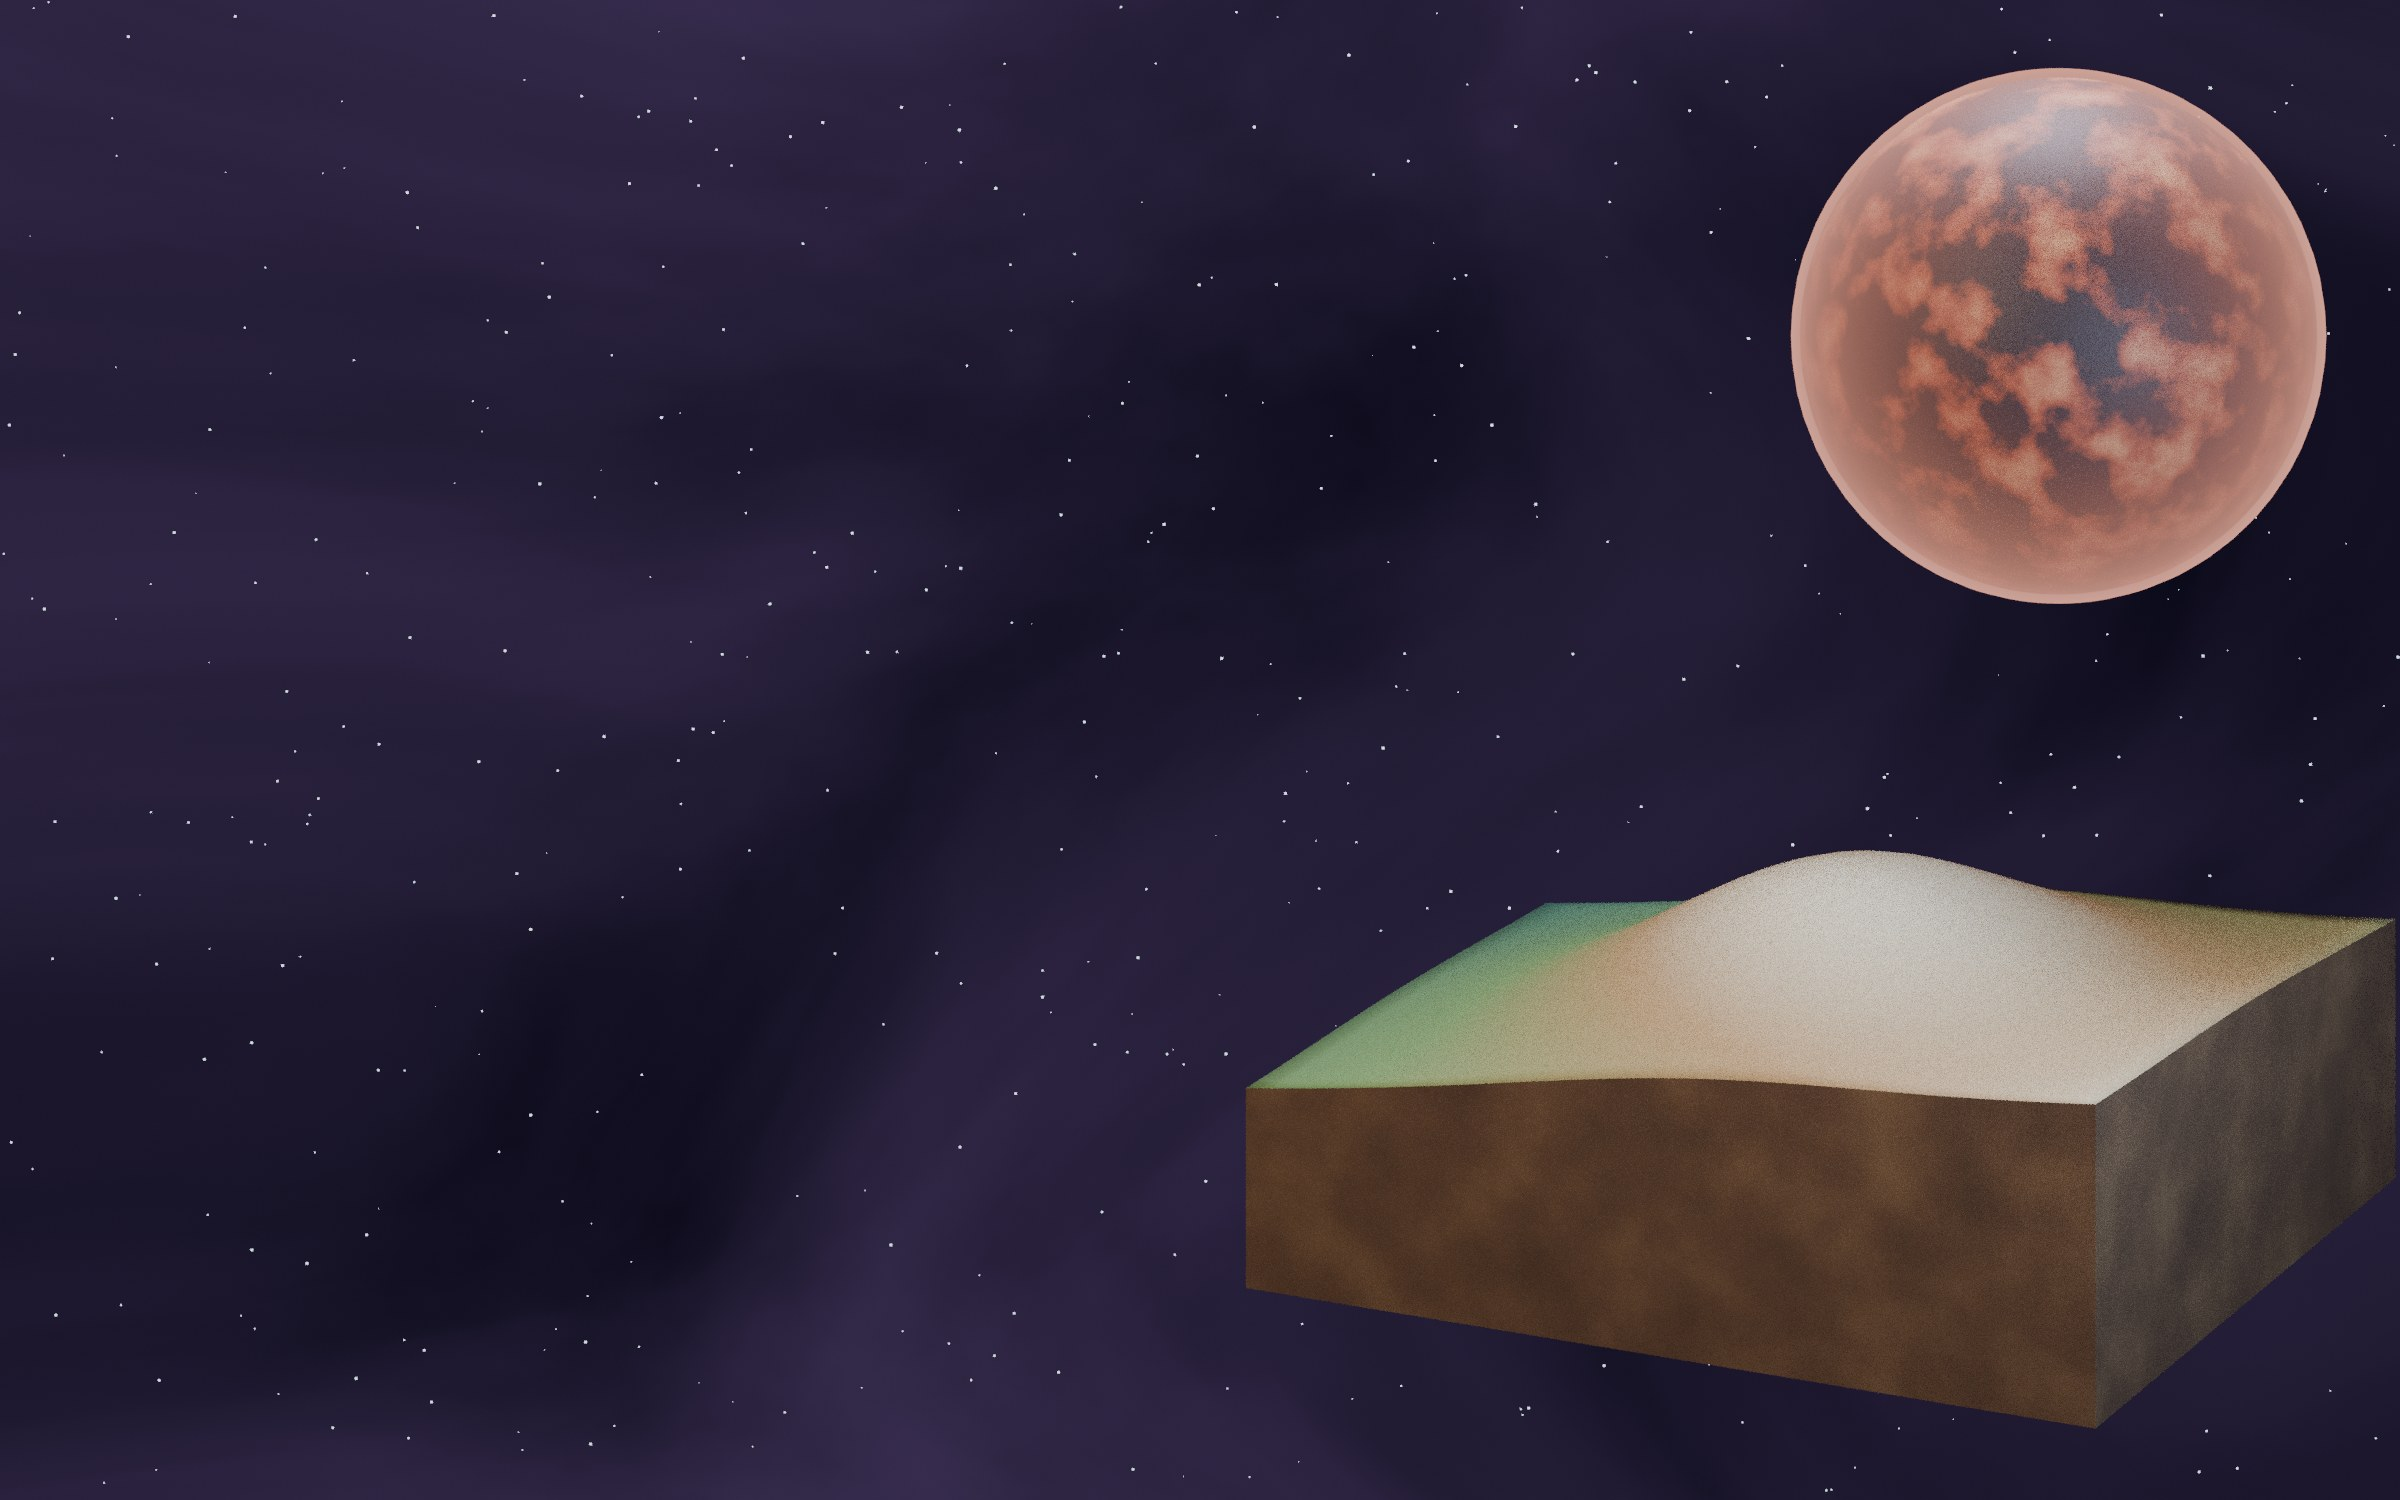
\includegraphics[width=20cm,height=12.5cm]{Scena/copertina.jpg}};}{}
\node[anchor=north west,inner sep=0] at([xshift=1.05cm,yshift=-1.10cm]current page.north west){\color{Mint}\bfseries\fontsize{23}{28}\selectfont SPEDIZIONE P07};
\node[anchor=north west,inner sep=0] at([xshift=1.07cm,yshift=-2.16cm]current page.north west){\color{white}\fontsize{9}{12}\selectfont MACROPROGETTO P07 · SCIENZE DELLA TERRA};
\draw[Mint,line width=1.5pt]([xshift=1.07cm,yshift=-2.78cm]current page.north west)--([xshift=2.6cm,yshift=-2.78cm]current page.north west);
\node[anchor=north west,inner sep=0] at([xshift=1.05cm,yshift=-3.35cm]current page.north west){\begin{minipage}{9.2cm}\raggedright\color{white}\bfseries\fontsize{28.5}{34.5}\selectfont Terreno, pendenze\\e sintesi\\territoriali\end{minipage}};
\node[anchor=north west,inner sep=0] at([xshift=1.07cm,yshift=-7.88cm]current page.north west){\begin{minipage}{8.9cm}\raggedright\color{Lilac}\fontsize{12.2}{17}\selectfont Un raster di 24 righe e 30 colonne\end{minipage}};
\node[anchor=north west,inner sep=0] at([xshift=1.07cm,yshift=-8.70cm]current page.north west){\begin{minipage}{8.9cm}\raggedright\color{white!75}\fontsize{10.3}{14.5}\selectfont Geometria raster, unità fisiche e ricampionamento di blocchi\end{minipage}};
\node[anchor=north west,inner sep=0] at([xshift=1.07cm,yshift=-10.52cm]current page.north west){\color{white}\fontsize{10.5}{14}\selectfont GeoStat Lab · corso di Marzio De Corato};
\node[anchor=north west,inner sep=0] at([xshift=1.07cm,yshift=-11.17cm]current page.north west){\color{Mint}\fontsize{8.8}{11}\selectfont\href{https://creativecommons.org/licenses/by-nc-sa/4.0/}{Impaginazione da Tessera · CC BY-NC-SA 4.0}};
\end{tikzpicture}\end{frame}

\begin{frame}[plain]\hypertarget{slide2}{}
\bookmark[level=1,page=2]{Indice della presentazione}
\begin{tikzpicture}[remember picture,overlay]
\PilotChrome{Indice della presentazione}{PERCORSO}{2}{I titoli dell’indice aprono i capitoli. Il nome del capitolo in alto riporta a questa pagina.}
\node[anchor=north west,inner sep=0] at([xshift=.96cm,yshift=-2.12cm]current page.north west){\Colonna{9.40cm}{\PLabel{Capitoli}
{\fontsize{10.7}{13.5}\selectfont\hyperlink{slide4}{Geometria e orientamento del raster\hfill 4}\par}\vspace{.16cm}
{\fontsize{10.7}{13.5}\selectfont\hyperlink{slide8}{Gradiente e pendenza fisica\hfill 8}\par}\vspace{.16cm}
{\fontsize{10.7}{13.5}\selectfont\hyperlink{slide12}{Zone e unità della sintesi\hfill 12}\par}\vspace{.16cm}
{\fontsize{10.7}{13.5}\selectfont\hyperlink{slide15}{Ricampionamento e limiti della conclusione\hfill 15}\par}\vspace{.16cm}
{\fontsize{10.7}{13.5}\selectfont\hyperlink{slide19}{Laboratori della spedizione\hfill 19}\par}\vspace{.16cm}

}};
\node[anchor=north west,inner sep=0] at([xshift=10.85cm,yshift=-2.12cm]current page.north west){\Colonna{8.16cm}{\PLabel{Percorso di lettura}
\PBody{Il percorso verifica geometria e orientamento del raster, deriva gradiente e pendenza fisica, sintetizza le zone con denominatori espliciti e discute il ricampionamento dei blocchi. I laboratori finali riprendono le tre fasi della spedizione.}
\PInfo{Le pagine Scenario A e Confronto riprendono gli esperimenti nel browser con dati sintetici. I valori di partenza del simulatore differiscono da quelli del caso.}
\href{https://marzione00.github.io/Lab_Geo/\#modulo-P07}{\color{Classical}\bfseries Apri la spedizione P07 su GeoStat Lab}
}};
\end{tikzpicture}\end{frame}

\begin{frame}[plain]\hypertarget{slide3}{}
\bookmark[level=1,page=3]{Quali quote e pendenze descrivono le due zone di un terreno sintetico, e che cosa misura un intervallo per la quota media?}
\begin{tikzpicture}[remember picture,overlay]
\PilotChrome{{\fontsize{15.3}{19}\selectfont Quali quote e pendenze descrivono le due zone di un terreno sintetico, e che cosa misura un intervallo per la quota media?}}{IL CASO GUIDA}{3}{La copertina è una scena illustrativa: il blocco di terreno riproduce le quote del raster.}
\node[anchor=north west,inner sep=0] at([xshift=.96cm,yshift=-2.12cm]current page.north west){\Colonna{9.40cm}{{\centering\resizebox{0.97\linewidth}{!}{\begin{tikzpicture}[x=1cm,y=1cm,every node/.style={font=\sffamily\fontsize{10}{12}\selectfont,text=Ink}]
\draw[draw=Classical,fill=Classical!8,rounded corners=2mm,line width=.7pt] (0,0.00) rectangle (8.6,-0.78);
\node[circle,anchor=center,fill=Classical,inner sep=0,minimum size=.5cm,text=white,font=\sffamily\bfseries\fontsize{9}{10}\selectfont] at (.48,-0.39) {1};
\node[anchor=west,text width=7.4cm,align=left] at (.95,-0.39) {Geometria e orientamento del raster};
\draw[pEdge] (.48,-0.80)--(.48,-1.02);
\draw[draw=Classical,fill=Classical!8,rounded corners=2mm,line width=.7pt] (0,-1.04) rectangle (8.6,-1.82);
\node[circle,anchor=center,fill=Classical,inner sep=0,minimum size=.5cm,text=white,font=\sffamily\bfseries\fontsize{9}{10}\selectfont] at (.48,-1.43) {2};
\node[anchor=west,text width=7.4cm,align=left] at (.95,-1.43) {Gradiente e pendenza fisica};
\draw[pEdge] (.48,-1.84)--(.48,-2.06);
\draw[draw=Classical,fill=Classical!8,rounded corners=2mm,line width=.7pt] (0,-2.08) rectangle (8.6,-2.86);
\node[circle,anchor=center,fill=Classical,inner sep=0,minimum size=.5cm,text=white,font=\sffamily\bfseries\fontsize{9}{10}\selectfont] at (.48,-2.47) {3};
\node[anchor=west,text width=7.4cm,align=left] at (.95,-2.47) {Zone e unità della sintesi};
\draw[pEdge] (.48,-2.88)--(.48,-3.10);
\draw[draw=Classical,fill=Classical!8,rounded corners=2mm,line width=.7pt] (0,-3.12) rectangle (8.6,-3.90);
\node[circle,anchor=center,fill=Classical,inner sep=0,minimum size=.5cm,text=white,font=\sffamily\bfseries\fontsize{9}{10}\selectfont] at (.48,-3.51) {4};
\node[anchor=west,text width=7.4cm,align=left] at (.95,-3.51) {Ricampionamento e limiti della conclusione};
\draw[pEdge] (.48,-3.92)--(.48,-4.14);
\draw[draw=GeoB,fill=GeoB!8,rounded corners=2mm,line width=.7pt] (0,-4.16) rectangle (8.6,-4.94);
\node[circle,anchor=center,fill=GeoB,inner sep=0,minimum size=.5cm,text=white,font=\sffamily\bfseries\fontsize{9}{10}\selectfont] at (.48,-4.55) {L};
\node[anchor=west,text width=7.4cm,align=left] at (.95,-4.55) {Laboratori della spedizione};
\end{tikzpicture}
}\par}
\PSmall{Capitoli della spedizione; L indica i laboratori conclusivi.}
}};
\node[anchor=north west,inner sep=0] at([xshift=10.85cm,yshift=-2.12cm]current page.north west){\Colonna{8.16cm}{\PLabel{Il caso}
\PBody{Un raster sintetico di 24 righe e 30 colonne, con celle quadrate di 30 metri, descrive una superficie liscia con georeferenziazione fittizia. Le celle vicine sono dipendenti, per cui il loro numero eccede quello delle repliche indipendenti.}
\PInfo{Seguiremo il raster dalla geometria alle pendenze in gradi, alle sintesi per zona e al ricampionamento di dodici blocchi.}
}};
\end{tikzpicture}\end{frame}

\begin{frame}[plain]\hypertarget{slide4}{}
\bookmark[level=0,page=4]{Geometria e orientamento del raster}
\bookmark[level=1,page=4]{La geometria della superficie sintetica}
\begin{tikzpicture}[remember picture,overlay]
\PilotChrome{La geometria della superficie sintetica}{GEOMETRIA E ORIENTAMENTO DEL RASTER}{4}{La geometria determina il significato fisico delle operazioni sulla matrice.}
\node[anchor=north west,inner sep=0] at([xshift=.96cm,yshift=-2.12cm]current page.north west){\Colonna{9.40cm}{{\centering\resizebox{0.90\linewidth}{!}{\begin{tikzpicture}[x=1cm,y=-.87cm,every node/.style={font=\fontsize{12.2}{15}\selectfont,text=Ink},arr/.style={-{Stealth[length=2mm]},line width=.8pt,draw=Classical}]\path[use as bounding box] (0,0) rectangle (7.45,6.2);
\draw[draw=Quantum,fill=Quantum!8,rounded corners=2pt,line width=.7pt] (0.7,1.0) rectangle (1.45,1.6);
\draw[draw=Classical,fill=Classical!8,rounded corners=2pt,line width=.7pt] (1.5,1.0) rectangle (2.25,1.6);
\draw[draw=Classical,fill=Classical!8,rounded corners=2pt,line width=.7pt] (2.3,1.0) rectangle (3.05,1.6);
\draw[draw=Quantum,fill=Quantum!8,rounded corners=2pt,line width=.7pt] (3.1000000000000005,1.0) rectangle (3.8500000000000005,1.6);
\draw[draw=Classical,fill=Classical!8,rounded corners=2pt,line width=.7pt] (3.9000000000000004,1.0) rectangle (4.65,1.6);
\draw[draw=Classical,fill=Classical!8,rounded corners=2pt,line width=.7pt] (4.7,1.0) rectangle (5.45,1.6);
\draw[draw=Quantum,fill=Quantum!8,rounded corners=2pt,line width=.7pt] (5.500000000000001,1.0) rectangle (6.250000000000001,1.6);
\draw[draw=Classical,fill=Classical!8,rounded corners=2pt,line width=.7pt] (0.7,1.65) rectangle (1.45,2.25);
\draw[draw=Classical,fill=Classical!8,rounded corners=2pt,line width=.7pt] (1.5,1.65) rectangle (2.25,2.25);
\draw[draw=Quantum,fill=Quantum!8,rounded corners=2pt,line width=.7pt] (2.3,1.65) rectangle (3.05,2.25);
\draw[draw=Classical,fill=Classical!8,rounded corners=2pt,line width=.7pt] (3.1000000000000005,1.65) rectangle (3.8500000000000005,2.25);
\draw[draw=Classical,fill=Classical!8,rounded corners=2pt,line width=.7pt] (3.9000000000000004,1.65) rectangle (4.65,2.25);
\draw[draw=Quantum,fill=Quantum!8,rounded corners=2pt,line width=.7pt] (4.7,1.65) rectangle (5.45,2.25);
\draw[draw=Classical,fill=Classical!8,rounded corners=2pt,line width=.7pt] (5.500000000000001,1.65) rectangle (6.250000000000001,2.25);
\draw[draw=Classical,fill=Classical!8,rounded corners=2pt,line width=.7pt] (0.7,2.3) rectangle (1.45,2.9000000000000004);
\draw[draw=Quantum,fill=Quantum!8,rounded corners=2pt,line width=.7pt] (1.5,2.3) rectangle (2.25,2.9000000000000004);
\draw[draw=Classical,fill=Classical!8,rounded corners=2pt,line width=.7pt] (2.3,2.3) rectangle (3.05,2.9000000000000004);
\draw[draw=Classical,fill=Classical!8,rounded corners=2pt,line width=.7pt] (3.1000000000000005,2.3) rectangle (3.8500000000000005,2.9000000000000004);
\draw[draw=Quantum,fill=Quantum!8,rounded corners=2pt,line width=.7pt] (3.9000000000000004,2.3) rectangle (4.65,2.9000000000000004);
\draw[draw=Classical,fill=Classical!8,rounded corners=2pt,line width=.7pt] (4.7,2.3) rectangle (5.45,2.9000000000000004);
\draw[draw=Classical,fill=Classical!8,rounded corners=2pt,line width=.7pt] (5.500000000000001,2.3) rectangle (6.250000000000001,2.9000000000000004);
\draw[draw=Quantum,fill=Quantum!8,rounded corners=2pt,line width=.7pt] (0.7,2.95) rectangle (1.45,3.5500000000000003);
\draw[draw=Classical,fill=Classical!8,rounded corners=2pt,line width=.7pt] (1.5,2.95) rectangle (2.25,3.5500000000000003);
\draw[draw=Classical,fill=Classical!8,rounded corners=2pt,line width=.7pt] (2.3,2.95) rectangle (3.05,3.5500000000000003);
\draw[draw=Quantum,fill=Quantum!8,rounded corners=2pt,line width=.7pt] (3.1000000000000005,2.95) rectangle (3.8500000000000005,3.5500000000000003);
\draw[draw=Classical,fill=Classical!8,rounded corners=2pt,line width=.7pt] (3.9000000000000004,2.95) rectangle (4.65,3.5500000000000003);
\draw[draw=Classical,fill=Classical!8,rounded corners=2pt,line width=.7pt] (4.7,2.95) rectangle (5.45,3.5500000000000003);
\draw[draw=Quantum,fill=Quantum!8,rounded corners=2pt,line width=.7pt] (5.500000000000001,2.95) rectangle (6.250000000000001,3.5500000000000003);
\draw[draw=Classical,fill=Classical!8,rounded corners=2pt,line width=.7pt] (0.7,3.6) rectangle (1.45,4.2);
\draw[draw=Classical,fill=Classical!8,rounded corners=2pt,line width=.7pt] (1.5,3.6) rectangle (2.25,4.2);
\draw[draw=Quantum,fill=Quantum!8,rounded corners=2pt,line width=.7pt] (2.3,3.6) rectangle (3.05,4.2);
\draw[draw=Classical,fill=Classical!8,rounded corners=2pt,line width=.7pt] (3.1000000000000005,3.6) rectangle (3.8500000000000005,4.2);
\draw[draw=Classical,fill=Classical!8,rounded corners=2pt,line width=.7pt] (3.9000000000000004,3.6) rectangle (4.65,4.2);
\draw[draw=Quantum,fill=Quantum!8,rounded corners=2pt,line width=.7pt] (4.7,3.6) rectangle (5.45,4.2);
\draw[draw=Classical,fill=Classical!8,rounded corners=2pt,line width=.7pt] (5.500000000000001,3.6) rectangle (6.250000000000001,4.2);
\node[anchor=center,text=Ink,font=\fontsize{11.5}{15}\selectfont,text width=6.8cm,align=center] at (3.7,0.3) {Schema di celle con valori e posizione};
\node[anchor=center,text=Ink,font=\fontsize{12}{15}\selectfont,text width=6.8cm,align=center] at (3.7,5.2) {Griglia effettiva: 24 × 30 celle};
\node[anchor=center,text=Ink,font=\fontsize{11.5}{15}\selectfont,text width=6.8cm,align=center] at (3.7,6) {30 m per lato; 64,8 ha};

\end{tikzpicture}}\par}
}};
\node[anchor=north west,inner sep=0] at([xshift=10.85cm,yshift=-2.12cm]current page.north west){\Colonna{8.16cm}{\PBody{Il progetto ricostruisce un terreno sintetico di ventiquattro righe e trenta colonne, con celle quadrate di trenta metri. L’obiettivo collega lettura del raster, calcolo delle pendenze, sintesi per zona e sensibilità al ricampionamento spaziale. La superficie liscia rende visibile la dipendenza fra celle vicine, per cui il loro numero non coincide con quello di repliche indipendenti. Il GeoTIFF conserva una georeferenziazione fittizia, che serve a esercitare il trattamento delle coordinate senza rappresentare un rilievo territoriale reale.}
}};
\end{tikzpicture}\end{frame}

\begin{frame}[plain]\hypertarget{slide5}{}
\bookmark[level=1,page=5]{Valori, estensione e sistema di riferimento}
\begin{tikzpicture}[remember picture,overlay]
\PilotChrome{Valori, estensione e sistema di riferimento}{GEOMETRIA E ORIENTAMENTO DEL RASTER}{5}{La corrispondenza dei valori deve essere verificata insieme all’orientamento degli assi.}
\node[anchor=north west,inner sep=0] at([xshift=.96cm,yshift=-2.12cm]current page.north west){\Colonna{9.40cm}{\PBody{La lettura del GeoTIFF verifica dimensioni, risoluzione, estensione e sistema di riferimento dichiarato. Le quote del file corrispondono a quelle della tabella CSV entro la precisione di memorizzazione, ma l’ordine delle righe è opposto: il raster procede dall’alto verso il basso, mentre la matrice locale segue y crescente. Il confronto richiede quindi un’inversione esplicita delle righe. Il controllo impedisce che una matrice numericamente plausibile venga associata a posizioni capovolte e mantiene dichiarata la natura fittizia della georeferenziazione.}
\par\smallskip{\centering\adjustbox{max width=.98\linewidth}{$\displaystyle Z^{GeoTIFF}_{r,c}\simeq Z^{locale}_{25-r,c}$}\par\smallskip}
}};
\node[anchor=north west,inner sep=0] at([xshift=10.85cm,yshift=-2.12cm]current page.north west){\Colonna{8.16cm}{\PInfo{r = 1,…,24 e c = 1,…,30: riga e colonna. Z contiene quote in metri; l’inversione r → 25 − r allinea gli orientamenti. Il GeoTIFF dichiara UTM 32N con estensione fittizia. La compatibilità numerica non dimostra una localizzazione reale né giustifica la sovrapposizione ai punti sintetici del progetto P06.}
}};
\end{tikzpicture}\end{frame}

\begin{frame}[plain]\hypertarget{slide6}{}
\bookmark[level=1,page=6]{Il confronto fra formati verifica la stessa superficie}
\begin{tikzpicture}[remember picture,overlay]
\PilotChrome{{\fontsize{15.3}{19}\selectfont Il confronto fra formati verifica la stessa superficie}}{GEOMETRIA E ORIENTAMENTO DEL RASTER}{6}{Un controllo fra formati deve specificare ordinamento, orientamento e tolleranza numerica.}
\node[anchor=north west,inner sep=0] at([xshift=.96cm,yshift=-2.12cm]current page.north west){\Colonna{9.40cm}{\PBody{Il frammento ordina le righe del CSV prima di ricostruire la matrice, poi confronta le quote con il GeoTIFF attraverso la convenzione di orientamento esplicitata. La tolleranza di un millesimo di metro ammette la differenza dovuta alla precisione numerica del formato, mantenendo il controllo molto più stretto delle variazioni del terreno. Dimensioni e passo vengono verificati separatamente, poiché l’uguaglianza di una sequenza di valori non sarebbe sufficiente a garantire la medesima geometria territoriale.}
}};
\node[anchor=north west,inner sep=0] at([xshift=10.85cm,yshift=-2.12cm]current page.north west){\Colonna{8.16cm}{\begin{tcolorbox}[enhanced,arc=1.7mm,boxrule=.6pt,colback=white,colframe=Classical!60!Navy,colbacktitle=Navy,coltitle=white,fonttitle=\bfseries\small,title={R · calcolo riproducibile},left=1.7mm,right=1.3mm,top=1.1mm,bottom=1.1mm,before skip=1mm,after skip=1.0mm]\lstinputlisting[style=GeoR,language=R,basicstyle=\ttfamily\fontsize{8.6}{11.4}\selectfont]{Codice/geometria.R}\end{tcolorbox}
\PLabel{Risultato in R}
\begin{tcolorbox}[colback=GeoTint,colframe=Rule,boxrule=.5pt,arc=1.4mm,left=2mm,right=1mm,top=1mm,bottom=1mm]{\fontsize{8.4}{10.9}\selectfont\ttfamily \mbox{[1]\ \ 901.0\ 1103.1}}\end{tcolorbox}
}};
\end{tikzpicture}\end{frame}

\begin{frame}[plain]\hypertarget{slide7}{}
\bookmark[level=1,page=7]{La carta delle quote e la scala metrica}
\begin{tikzpicture}[remember picture,overlay]
\PilotChrome{La carta delle quote e la scala metrica}{GEOMETRIA E ORIENTAMENTO DEL RASTER}{7}{Risoluzione e supporto della cella delimitano le strutture interpretabili nella superficie.}
\node[anchor=north west,inner sep=0] at([xshift=.96cm,yshift=-2.12cm]current page.north west){\Colonna{9.40cm}{{\centering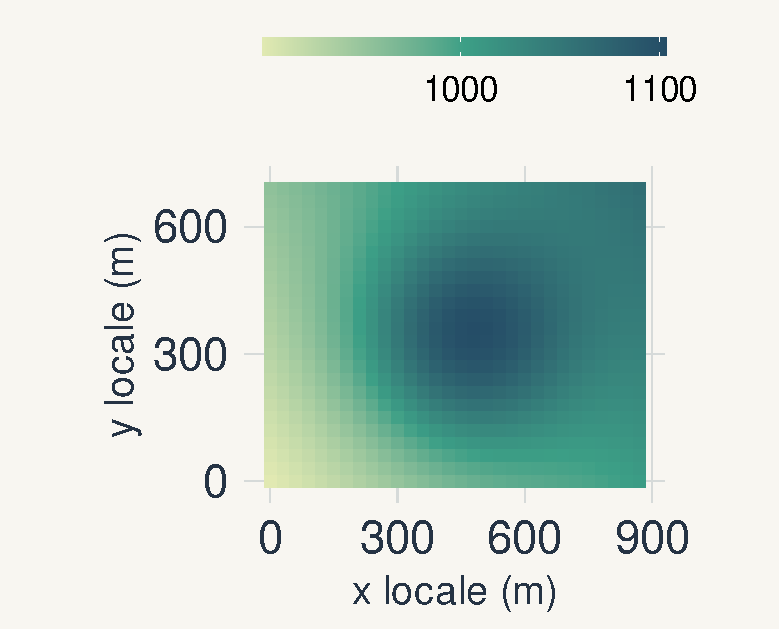
\includegraphics[width=\linewidth,height=6.15cm,keepaspectratio]{Figure/F01.pdf}\par}
\PSmall{Quote sintetiche sulla griglia locale di trenta metri.}
}};
\node[anchor=north west,inner sep=0] at([xshift=10.85cm,yshift=-2.12cm]current page.north west){\Colonna{8.16cm}{\PBody{La superficie viene rappresentata con rapporto unitario fra gli assi e una scala cromatica continua della quota. Ogni cella conserva il proprio supporto areale di novecento metri quadrati, mentre i valori rappresentano il terreno sintetico campionato sulla griglia. La carta permette di riconoscere variazioni graduali e direzioni di cambiamento, che verranno riassunte attraverso il gradiente. La risoluzione della griglia limita le strutture rappresentabili e deve accompagnare l’interpretazione delle derivate calcolate numericamente.}
}};
\end{tikzpicture}\end{frame}

\begin{frame}[plain]\hypertarget{slide8}{}
\bookmark[level=0,page=8]{Gradiente e pendenza fisica}
\bookmark[level=1,page=8]{Le differenze centrate approssimano il gradiente}
\begin{tikzpicture}[remember picture,overlay]
\PilotChrome{Le differenze centrate approssimano il gradiente}{GRADIENTE E PENDENZA FISICA}{8}{Il denominatore della differenza finita è una distanza fisica, determinata dalla risoluzione.}
\node[anchor=north west,inner sep=0] at([xshift=.96cm,yshift=-2.12cm]current page.north west){\Colonna{9.40cm}{{\centering\resizebox{0.90\linewidth}{!}{\begin{tikzpicture}[x=1cm,y=-.87cm,every node/.style={font=\fontsize{12.2}{15}\selectfont,text=Ink},arr/.style={-{Stealth[length=2mm]},line width=.8pt,draw=Classical}]\path[use as bounding box] (0,0) rectangle (7.45,6.2);
\draw[draw=Quantum,fill=Quantum!8,rounded corners=2pt,line width=.7pt] (2.6,2.1) rectangle (4.2,3.7);
\node[anchor=center,text=Ink,font=\fontsize{14}{15}\selectfont] at (3.4,2.9) {$Z_{r,c}$};
\draw[draw=Classical,fill=Classical!8,rounded corners=2pt,line width=.7pt] (0.6,2.1) rectangle (2.2,3.7);
\node[anchor=center,text=Ink,font=\fontsize{12}{15}\selectfont] at (1.4,2.9) {$Z_{r,c-1}$};
\draw[draw=Classical,fill=Classical!8,rounded corners=2pt,line width=.7pt] (4.6,2.1) rectangle (6.2,3.7);
\node[anchor=center,text=Ink,font=\fontsize{12}{15}\selectfont] at (5.4,2.9) {$Z_{r,c+1}$};
\draw[arr,draw=Classical] (0.7,4.5)--(6.1,4.5);
\node[anchor=center,text=Ink,font=\fontsize{11.5}{15}\selectfont,text width=6.5cm,align=center] at (3.4,5.3) {Distanza fra i due vicini: 60 m};
\node[anchor=center,text=Ink,font=\fontsize{11.5}{15}\selectfont,text width=6.8cm,align=center] at (3.7,0.9) {Derivata lungo x nella cella centrale};

\end{tikzpicture}}\par}
\PSmall{$Z_{r,c}$: quota in metri; r cresce con y, c con x; $\Delta x=\Delta y=30$ m. $g_x,g_y$: derivate in m/m.}
}};
\node[anchor=north west,inner sep=0] at([xshift=10.85cm,yshift=-2.12cm]current page.north west){\Colonna{8.16cm}{\PBody{Nelle celle interne, la derivata rispetto a x viene approssimata confrontando le due celle laterali, separate da sessanta metri; lo stesso procedimento viene applicato lungo y. Le differenze centrate utilizzano così una finestra locale e producono componenti del gradiente in metri per metro. Le celle del bordo vengono escluse, poiché il loro calcolo richiederebbe una regola differente o valori esterni alla griglia. Rimangono ventidue righe per ventotto colonne, pari a 616 pendenze interne.}
\par\smallskip{\centering\adjustbox{max width=.98\linewidth}{$\displaystyle g_x\simeq\frac{Z_{r,c+1}-Z_{r,c-1}}{2\Delta x},\qquad g_y\simeq\frac{Z_{r+1,c}-Z_{r-1,c}}{2\Delta y}$}\par\smallskip}
}};
\end{tikzpicture}\end{frame}

\begin{frame}[plain]\hypertarget{slide9}{}
\bookmark[level=1,page=9]{Angolo e percentuale derivano dalla stessa tangente}
\begin{tikzpicture}[remember picture,overlay]
\PilotChrome{{\fontsize{15.3}{19}\selectfont Angolo e percentuale derivano dalla stessa tangente}}{GRADIENTE E PENDENZA FISICA}{9}{L’angolo e la percentuale esprimono la stessa inclinazione attraverso scale differenti.}
\node[anchor=north west,inner sep=0] at([xshift=.96cm,yshift=-2.12cm]current page.north west){\Colonna{9.40cm}{{\centering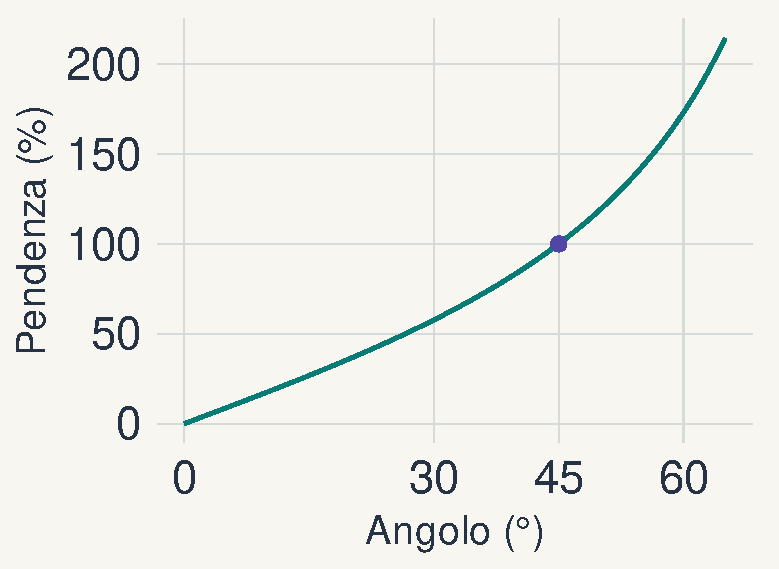
\includegraphics[width=\linewidth,height=6.15cm,keepaspectratio]{Figure/F03.pdf}\par}
\PSmall{$g_x,g_y$: derivate della quota; g: norma, in m/m; $\theta$: gradi; $p_\%$: percentuale. Punto viola: 45° = 100\%.}
}};
\node[anchor=north west,inner sep=0] at([xshift=10.85cm,yshift=-2.12cm]current page.north west){\Colonna{8.16cm}{\PBody{La norma del gradiente esprime il rapporto fra variazione verticale e distanza orizzontale nella direzione di massima crescita. Coincidendo con la tangente della pendenza, permette di ricavarne angolo e percentuale. La percentuale è cento volte il rapporto, mentre l’angolo richiede l’arcotangente e la conversione da radianti a gradi. Un angolo di quarantacinque gradi corrisponde quindi al cento per cento, come viene verificato numericamente nel codice.}
\par\smallskip{\centering\adjustbox{max width=.98\linewidth}{$\displaystyle \begin{gathered}g=\sqrt{g_x^2+g_y^2},\qquad\theta=\arctan(g)\frac{180}{\pi}\\p_{\%}=100g=100\tan\!\left(\theta\frac{\pi}{180}\right)\end{gathered}$}\par\smallskip}
}};
\end{tikzpicture}\end{frame}

\begin{frame}[plain]\hypertarget{slide10}{}
\bookmark[level=1,page=10]{Il codice conserva dominio e unità delle derivate}
\begin{tikzpicture}[remember picture,overlay]
\PilotChrome{Il codice conserva dominio e unità delle derivate}{GRADIENTE E PENDENZA FISICA}{10}{Le verifiche numeriche collegano il calcolo matriciale alla definizione geometrica della pendenza.}
\node[anchor=north west,inner sep=0] at([xshift=.96cm,yshift=-2.12cm]current page.north west){\Colonna{9.40cm}{\PBody{Le porzioni della matrice vengono selezionate in modo da confrontare celle simmetriche attorno a ogni posizione interna. Il calcolo produce matrici di dimensione identica per le due derivate, delle quali si combina la norma prima della trasformazione in gradi. Il controllo inverso riconduce l’angolo alla pendenza percentuale e intercetta errori di conversione. Una prova supplementare su un piano di pendenza nota, sviluppata nel modulo M12, verifica che il metodo recuperi le componenti imposte analiticamente.}
}};
\node[anchor=north west,inner sep=0] at([xshift=10.85cm,yshift=-2.12cm]current page.north west){\Colonna{8.16cm}{\begin{tcolorbox}[enhanced,arc=1.7mm,boxrule=.6pt,colback=white,colframe=Classical!60!Navy,colbacktitle=Navy,coltitle=white,fonttitle=\bfseries\small,title={R · calcolo riproducibile},left=1.7mm,right=1.3mm,top=1.1mm,bottom=1.1mm,before skip=1mm,after skip=1.0mm]\lstinputlisting[style=GeoR,language=R,basicstyle=\ttfamily\fontsize{8.6}{11.4}\selectfont]{Codice/pendenza.R}\end{tcolorbox}
\PLabel{Risultato in R}
\begin{tcolorbox}[colback=GeoTint,colframe=Rule,boxrule=.5pt,arc=1.4mm,left=2mm,right=1mm,top=1mm,bottom=1mm]{\fontsize{8.4}{10.9}\selectfont\ttfamily \mbox{[1]\ \ 0.49\ 28.53}}\end{tcolorbox}
}};
\end{tikzpicture}\end{frame}

\begin{frame}[plain]\hypertarget{slide11}{}
\bookmark[level=1,page=11]{La carta delle pendenze riguarda soltanto l’interno}
\begin{tikzpicture}[remember picture,overlay]
\PilotChrome{{\fontsize{15.3}{19}\selectfont La carta delle pendenze riguarda soltanto l’interno}}{GRADIENTE E PENDENZA FISICA}{11}{Una derivata raster viene interpretata rispetto a risoluzione, finestra e trattamento del bordo.}
\node[anchor=north west,inner sep=0] at([xshift=.96cm,yshift=-2.12cm]current page.north west){\Colonna{9.40cm}{{\centering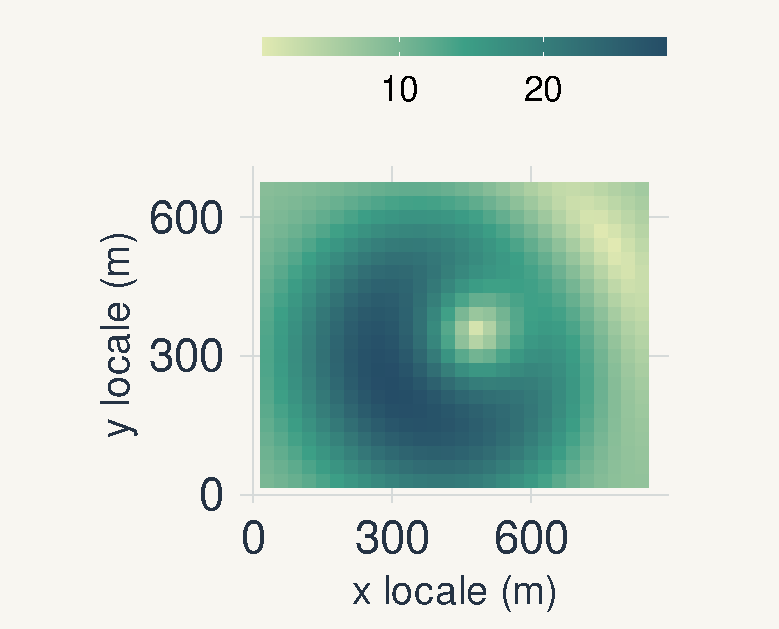
\includegraphics[width=\linewidth,height=6.15cm,keepaspectratio]{Figure/F02.pdf}\par}
\PSmall{Pendenza in gradi nelle 616 celle interne.}
}};
\node[anchor=north west,inner sep=0] at([xshift=10.85cm,yshift=-2.12cm]current page.north west){\Colonna{8.16cm}{\PBody{Le 616 celle interne mostrano pendenze comprese fra circa 0,49 e 28,53 gradi. La rappresentazione rende riconoscibili zone di maggiore inclinazione, mantenendo il bordo escluso dal calcolo. La derivata amplifica variazioni locali e dipende dal passo e dalla regola numerica adottati; una diversa risoluzione potrebbe quindi modificare il risultato anche descrivendo lo stesso terreno generale. L’interpretazione collega la carta all’algoritmo e alla geometria, evitando di considerare ogni valore una proprietà indipendente dalla scala di osservazione.}
}};
\end{tikzpicture}\end{frame}

\begin{frame}[plain]\hypertarget{slide12}{}
\bookmark[level=0,page=12]{Zone e unità della sintesi}
\bookmark[level=1,page=12]{L’aggregazione produce una riga per zona}
\begin{tikzpicture}[remember picture,overlay]
\PilotChrome{L’aggregazione produce una riga per zona}{ZONE E UNITÀ DELLA SINTESI}{12}{L’unità della tabella aggregata e il numero delle repliche inferenziali devono essere dichiarati separatamente.}
\node[anchor=north west,inner sep=0] at([xshift=.96cm,yshift=-2.12cm]current page.north west){\Colonna{9.40cm}{{\centering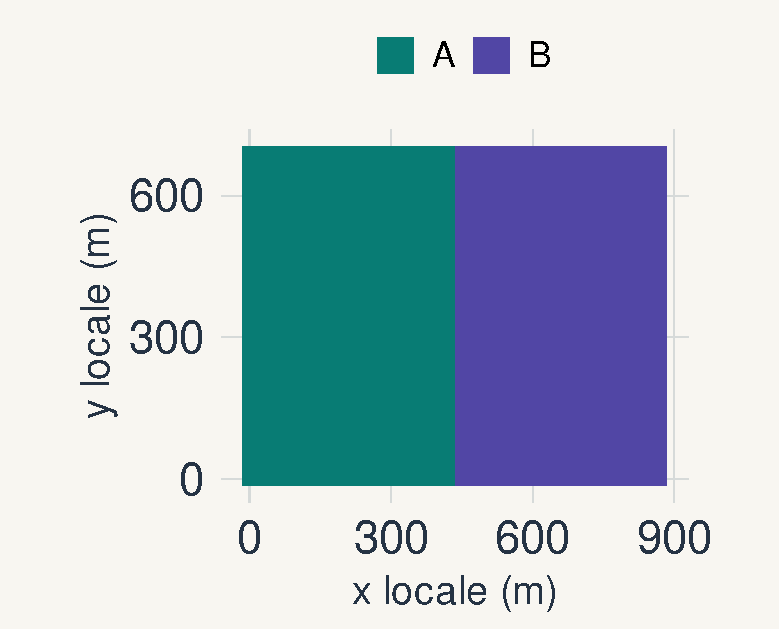
\includegraphics[width=\linewidth,height=6.15cm,keepaspectratio]{Figure/F04.pdf}\par}
\PSmall{Due zone sintetiche di 360 celle e 32,4 ettari ciascuna.}
}};
\node[anchor=north west,inner sep=0] at([xshift=10.85cm,yshift=-2.12cm]current page.north west){\Colonna{8.16cm}{\PBody{La griglia è suddivisa in due zone sintetiche, A e B, ciascuna composta da 360 celle. La sintesi riunisce le quote entro ogni zona e produce una tabella con media, deviazione standard, conteggio e area. Il passaggio modifica il livello della tabella: la riga finale rappresenta una zona, mentre il conteggio delle celle descrive copertura e risoluzione. La regolarità spaziale del terreno rende improprio interpretare automaticamente le 360 celle come altrettante repliche indipendenti per un confronto inferenziale.}
}};
\end{tikzpicture}\end{frame}

\begin{frame}[plain]\hypertarget{slide13}{}
\bookmark[level=1,page=13]{Media zonale e area hanno denominatori espliciti}
\begin{tikzpicture}[remember picture,overlay]
\PilotChrome{Media zonale e area hanno denominatori espliciti}{ZONE E UNITÀ DELLA SINTESI}{13}{La sintesi territoriale richiede pesi coerenti con area, copertura e supporto della variabile.}
\node[anchor=north west,inner sep=0] at([xshift=.96cm,yshift=-2.12cm]current page.north west){\Colonna{9.40cm}{\PBody{Le celle hanno area uguale, per cui la media aritmetica coincide con la media pesata per area della rappresentazione raster. La zona A ha quota media circa 986,025 metri e la zona B circa 1044,597 metri; le deviazioni standard descrittive sono circa 46,018 e 27,345 metri. L’area di ciascuna zona è 32,4 ettari. Con celle di area diversa o copertura incompleta, la ponderazione e il denominatore richiederebbero una formulazione ulteriore, coerente con la quantità territoriale da rappresentare.}
\par\smallskip{\centering\adjustbox{max width=.98\linewidth}{$\displaystyle \begin{gathered}\overline z_A=\frac{\sum_{i\in A}a_i z_i}{\sum_{i\in A}a_i},\qquad a_i=900\ \mathrm{m^2}\\\mathrm{area}(A)=360\times900/10^4=32{,}4\ \mathrm{ha}\end{gathered}$}\par\smallskip}
}};
\node[anchor=north west,inner sep=0] at([xshift=10.85cm,yshift=-2.12cm]current page.north west){\Colonna{8.16cm}{\PInfo{$z_i$: quota della cella i, in m; $a_i$: area della cella; A: insieme delle celle della zona. Le due medie descrivono la superficie disponibile. Un intervallo inferenziale sulla differenza richiederebbe un processo generatore, un disegno di osservazione e una rappresentazione della dipendenza.}
}};
\end{tikzpicture}\end{frame}

\begin{frame}[plain]\hypertarget{slide14}{}
\bookmark[level=1,page=14]{La dispersione spaziale delle quote}
\begin{tikzpicture}[remember picture,overlay]
\PilotChrome{La dispersione spaziale delle quote}{ZONE E UNITÀ DELLA SINTESI}{14}{La variabilità nello spazio e l’incertezza su una media sono quantità differenti.}
\node[anchor=north west,inner sep=0] at([xshift=.96cm,yshift=-2.12cm]current page.north west){\Colonna{9.40cm}{{\centering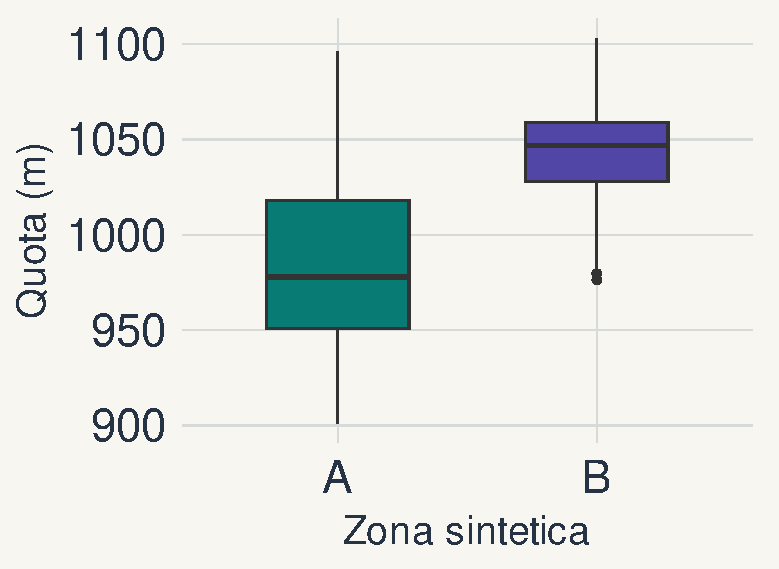
\includegraphics[width=\linewidth,height=6.15cm,keepaspectratio]{Figure/F05.pdf}\par}
\PSmall{Distribuzioni delle quote nelle due zone; scatole descrittive delle celle.}
}};
\node[anchor=north west,inner sep=0] at([xshift=10.85cm,yshift=-2.12cm]current page.north west){\Colonna{8.16cm}{\PBody{I boxplot confrontano la distribuzione delle quote nelle due zone, rendendo visibili differenze di livello e dispersione. Le scatole riassumono valori delle celle e non costituiscono intervalli di confidenza delle medie zonali. La maggiore variabilità della zona A descrive la superficie campionata, senza implicare da sola maggiore incertezza strumentale. La distinzione fra eterogeneità territoriale, errore di misura e incertezza inferenziale rimane essenziale quando una carta viene trasformata in una tabella di sintesi.}
}};
\end{tikzpicture}\end{frame}

\begin{frame}[plain]\hypertarget{slide15}{}
\bookmark[level=0,page=15]{Ricampionamento e limiti della conclusione}
\bookmark[level=1,page=15]{La struttura locale nei blocchi}
\begin{tikzpicture}[remember picture,overlay]
\PilotChrome{La struttura locale nei blocchi}{RICAMPIONAMENTO E LIMITI DELLA CONCLUSIONE}{15}{La dimensione dei blocchi deve essere discussa rispetto alla scala della dipendenza spaziale.}
\node[anchor=north west,inner sep=0] at([xshift=.96cm,yshift=-2.12cm]current page.north west){\Colonna{9.40cm}{{\centering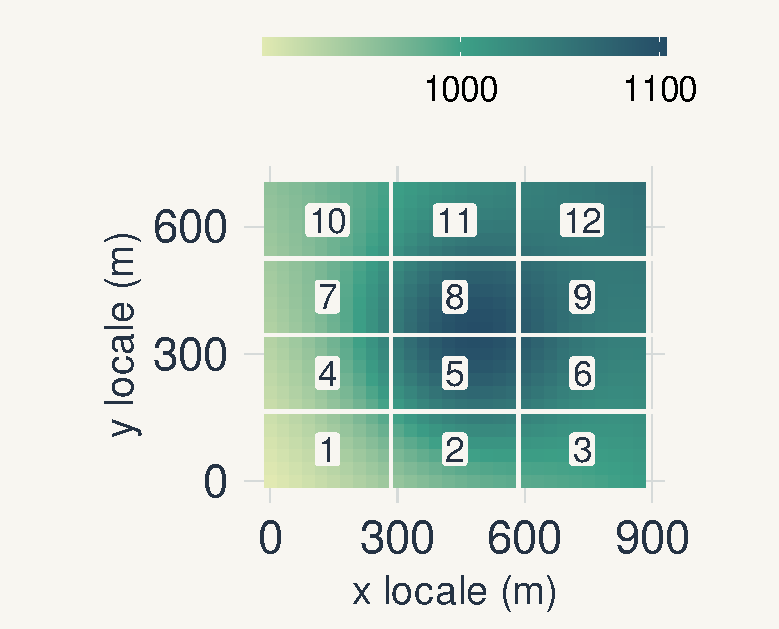
\includegraphics[width=\linewidth,height=6.15cm,keepaspectratio]{Figure/F06.pdf}\par}
\PSmall{Dodici blocchi di 6 × 10 celle, identificati sulla superficie.}
}};
\node[anchor=north west,inner sep=0] at([xshift=10.85cm,yshift=-2.12cm]current page.north west){\Colonna{8.16cm}{\PBody{Il terreno viene suddiviso in dodici blocchi contigui, ciascuno di sei righe per dieci colonne. La media di ogni blocco riassume sessanta celle e viene utilizzata come unità del ricampionamento. Poiché i blocchi hanno la stessa area, la media delle dodici medie coincide con quella delle 720 celle, circa 1015,311 metri. La scelta conserva una struttura locale più ampia rispetto al ricampionamento delle singole celle, pur lasciando possibile dipendenza fra blocchi confinanti.}
}};
\end{tikzpicture}\end{frame}

\begin{frame}[plain]\hypertarget{slide16}{}
\bookmark[level=1,page=16]{La replica estrae dodici medie di blocco}
\begin{tikzpicture}[remember picture,overlay]
\PilotChrome{La replica estrae dodici medie di blocco}{RICAMPIONAMENTO E LIMITI DELLA CONCLUSIONE}{16}{L’unità ricampionata esprime un’ipotesi sulla componente di variabilità rappresentata.}
\node[anchor=north west,inner sep=0] at([xshift=.96cm,yshift=-2.12cm]current page.north west){\Colonna{9.40cm}{{\centering\resizebox{0.90\linewidth}{!}{\begin{tikzpicture}[x=1cm,y=-.87cm,every node/.style={font=\fontsize{12.2}{15}\selectfont,text=Ink},arr/.style={-{Stealth[length=2mm]},line width=.8pt,draw=Classical}]\path[use as bounding box] (0,0) rectangle (7.45,6.2);
\draw[draw=Classical,fill=Classical!8,rounded corners=2pt,line width=.7pt] (0.6,0.8) rectangle (6.8,2.2);
\node[anchor=center,text=Ink,font=\fontsize{13}{15}\selectfont,text width=5.8cm,align=center] at (3.7,1.5) {Dodici blocchi osservati};
\draw[arr,draw=Quantum] (3.7,2.5)--(3.7,3.2);
\draw[draw=Quantum,fill=Quantum!8,rounded corners=2pt,line width=.7pt] (0.6,3.5) rectangle (6.8,4.9);
\node[anchor=center,text=Ink,font=\fontsize{12}{15}\selectfont,text width=5.8cm,align=center] at (3.7,4.2) {Dodici estrazioni con reinserimento};
\node[anchor=center,text=Ink,font=\fontsize{11.5}{15}\selectfont,text width=6.7cm,align=center] at (3.7,5.8) {Le molteplicità cambiano fra le repliche.};

\end{tikzpicture}}\par}
\PSmall{$z_i$: quota di cella; b: blocco di 60 celle. Gli indici $I_r$ sono estratti indipendentemente e uniformemente da 1,…,12, con reinserimento.}
}};
\node[anchor=north west,inner sep=0] at([xshift=10.85cm,yshift=-2.12cm]current page.north west){\Colonna{8.16cm}{\PBody{Ogni replica seleziona con reinserimento dodici medie di blocco e ne calcola la media. La procedura produce 1999 repliche e conserva il piano degli indici utilizzati, rendendo ricostruibile ogni estrazione. Il riferimento tratta i blocchi osservati come unità scambiabili, ipotesi che richiede cautela su una superficie liscia e con struttura territoriale. L’esercizio viene interpretato come sensibilità condizionata allo schema, mentre un intervallo con validità generale richiederebbe una giustificazione probabilistica della disposizione e della dimensione dei blocchi.}
\par\smallskip{\centering\adjustbox{max width=.98\linewidth}{$\displaystyle \overline z_b=\frac1{60}\sum_{i\in b}z_i,\qquad\overline z^{*}=\frac1{12}\sum_{r=1}^{12}\overline z_{I_r}$}\par\smallskip}
}};
\end{tikzpicture}\end{frame}

\begin{frame}[plain]\hypertarget{slide17}{}
\bookmark[level=1,page=17]{L’intervallo descrive il riferimento adottato}
\begin{tikzpicture}[remember picture,overlay]
\PilotChrome{L’intervallo descrive il riferimento adottato}{RICAMPIONAMENTO E LIMITI DELLA CONCLUSIONE}{17}{L’incertezza richiede un bersaglio probabilistico; la media di un raster completo è una quantità finita osservata.}
\node[anchor=north west,inner sep=0] at([xshift=.96cm,yshift=-2.12cm]current page.north west){\Colonna{9.40cm}{{\centering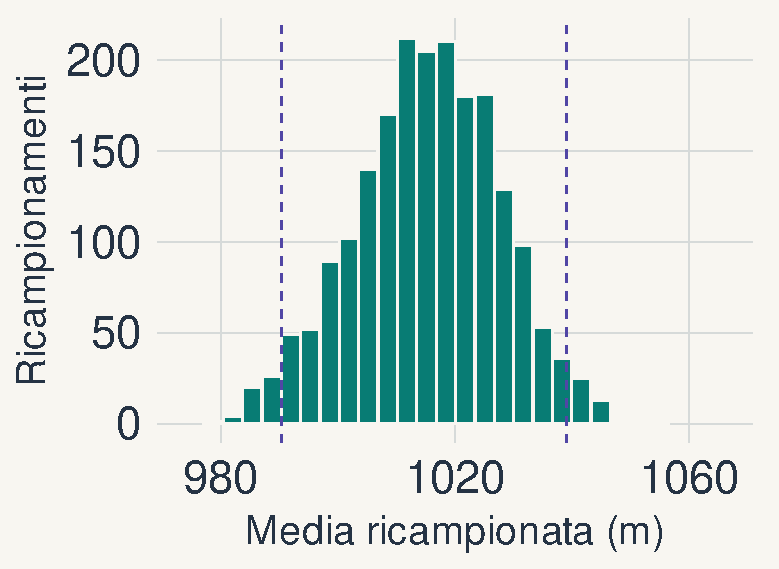
\includegraphics[width=\linewidth,height=6.15cm,keepaspectratio]{Figure/F07.pdf}\par}
\PSmall{Distribuzione di 1999 medie ricampionate; linee viola: quantili percentili.}
}};
\node[anchor=north west,inner sep=0] at([xshift=10.85cm,yshift=-2.12cm]current page.north west){\Colonna{8.16cm}{\PBody{I quantili 2,5\% e 97,5\% delle medie ricampionate sono circa 990,284 e 1038,958 metri. L’ampiezza riflette la variabilità fra i dodici blocchi osservati sotto la procedura definita, mentre la media della superficie completa è già calcolabile esattamente dai valori disponibili. Il ricampionamento non misura automaticamente l’errore di quella media finita. La distinzione diventa particolarmente rilevante se si vuole estendere l’argomento a un processo territoriale, ad altre aree o a una raccolta incompleta di osservazioni.}
}};
\end{tikzpicture}\end{frame}

\begin{frame}[plain]\hypertarget{slide18}{}
\bookmark[level=1,page=18]{Consegna e interpretazione territoriale}
\begin{tikzpicture}[remember picture,overlay]
\PilotChrome{Consegna e interpretazione territoriale}{RICAMPIONAMENTO E LIMITI DELLA CONCLUSIONE}{18}{Il significato fisico e inferenziale dei risultati dipende dalla geometria e dall’unità della sintesi.}
\node[anchor=north west,inner sep=0] at([xshift=.96cm,yshift=-2.12cm]current page.north west){\Colonna{9.40cm}{\PBody{La relazione conserva audit del GeoTIFF, confronto dell’orientamento, formula delle pendenze, statistiche zonali, disposizione dei blocchi e distribuzione ricampionata. L’esercizio richiede di spiegare perché quarantacinque gradi corrispondano al cento per cento e perché 360 celle non garantiscano 360 repliche indipendenti. Una discussione finale individua quale bersaglio potrebbe giustificare un’inferenza oltre la superficie completa disponibile. La conclusione collega ogni grandezza al supporto spaziale, alle unità e alla natura sintetica dei dati.}
}};
\node[anchor=north west,inner sep=0] at([xshift=10.85cm,yshift=-2.12cm]current page.north west){\Colonna{8.16cm}{\PInfo{R/P07\_figure.R integra le attività M12\_N03, N10, N15 e N17. Il progetto utilizza 1999 repliche e conserva i piani di estrazione. GeoTIFF e CSV sono accompagnati dai metadati e dalle verifiche di orientamento, affinché la riproduzione comprenda sia i valori sia la loro collocazione spaziale.}
}};
\end{tikzpicture}\end{frame}

\begin{frame}[plain]\hypertarget{slide19}{}
\bookmark[level=0,page=19]{Laboratori della spedizione}
\bookmark[level=1,page=19]{Tre fasi della spedizione nel laboratorio}
\begin{tikzpicture}[remember picture,overlay]
\PilotChrome{Tre fasi della spedizione nel laboratorio}{LABORATORI DELLA SPEDIZIONE}{19}{Gli esperimenti usano griglie sintetiche; la conclusione sul caso resta quella ottenuta dal raster della spedizione.}
\node[anchor=north west,inner sep=0] at([xshift=.96cm,yshift=-2.12cm]current page.north west){\Colonna{9.40cm}{{\centering\resizebox{0.97\linewidth}{!}{\begin{tikzpicture}[x=1cm,y=1cm,every node/.style={font=\sffamily\fontsize{9.2}{11}\selectfont,text=Ink}]
\node[draw=Classical,fill=Classical,rounded corners=2mm,text=white,text width=2.45cm,align=flush center,minimum height=1.55cm,anchor=west,font=\sffamily\bfseries\fontsize{9.2}{11}\selectfont] (f0) at (0,0.00) {1. Verificare la griglia};
\node[draw=Classical!60,fill=Classical!6,rounded corners=1.5mm,line width=.6pt,text width=2.8cm,align=flush center,minimum height=1.55cm,anchor=west] (e00) at (2.95,0.00) {Geometria di una griglia raster\\[1pt]{\fontsize{7.6}{9}\selectfont\color{Muted}m12-griglia}};
\node[draw=Rule,fill=white,rounded corners=1.5mm,line width=.6pt,text width=2.8cm,align=flush center,minimum height=1.55cm,anchor=west] (e01) at (6.10,0.00) {Maschere, dominio e superficie valida\\[1pt]{\fontsize{7.6}{9}\selectfont\color{Muted}m12-maschere}};
\draw[pEdge] (f0.east)--(e00.west);
\node[draw=Classical,fill=Classical,rounded corners=2mm,text=white,text width=2.45cm,align=flush center,minimum height=1.55cm,anchor=west,font=\sffamily\bfseries\fontsize{9.2}{11}\selectfont] (f1) at (0,-1.95) {2. Derivare e rappresentare};
\draw[pEdge] (f0.south)--(f1.north);
\node[draw=Classical!60,fill=Classical!6,rounded corners=1.5mm,line width=.6pt,text width=2.8cm,align=flush center,minimum height=1.55cm,anchor=west] (e10) at (2.95,-1.95) {Gradiente, pendenza ed esposizione\\[1pt]{\fontsize{7.6}{9}\selectfont\color{Muted}m12-pendenza}};
\node[draw=Rule,fill=white,rounded corners=1.5mm,line width=.6pt,text width=2.8cm,align=flush center,minimum height=1.55cm,anchor=west] (e11) at (6.10,-1.95) {Illuminazione del rilievo\\[1pt]{\fontsize{7.6}{9}\selectfont\color{Muted}m12-hillshade}};
\draw[pEdge] (f1.east)--(e10.west);
\node[draw=Classical,fill=Classical,rounded corners=2mm,text=white,text width=2.45cm,align=flush center,minimum height=1.55cm,anchor=west,font=\sffamily\bfseries\fontsize{9.2}{11}\selectfont] (f2) at (0,-3.90) {3. Valutare la sensibilità};
\draw[pEdge] (f1.south)--(f2.north);
\node[draw=Classical!60,fill=Classical!6,rounded corners=1.5mm,line width=.6pt,text width=2.8cm,align=flush center,minimum height=1.55cm,anchor=west] (e20) at (2.95,-3.90) {Aggregazione e ricampionamento di una griglia\\[1pt]{\fontsize{7.6}{9}\selectfont\color{Muted}m12-ricampionamento}};
\node[draw=Rule,fill=white,rounded corners=1.5mm,line width=.6pt,text width=2.8cm,align=flush center,minimum height=1.55cm,anchor=west] (e21) at (6.10,-3.90) {Allineamento e ricampionamento fra griglie\\[1pt]{\fontsize{7.6}{9}\selectfont\color{Muted}m12-allineamento}};
\draw[pEdge] (f2.east)--(e20.west);
\end{tikzpicture}
}\par}
\PSmall{Fasi della spedizione. Il primo esperimento di ogni fase ha le pagine Scenario A e Confronto.}
}};
\node[anchor=north west,inner sep=0] at([xshift=10.85cm,yshift=-2.12cm]current page.north west){\Colonna{8.16cm}{\PBody{Gli esperimenti ripetono su griglie sintetiche tre passaggi della spedizione: leggere la geometria della griglia, derivare pendenza ed esposizione, aggregare le celle in blocchi. Ogni fase ha uno scenario di partenza e un confronto con un solo parametro modificato.}
\vspace{.2cm}\PLabel{Altri esperimenti delle fasi}
\PLab{https://marzione00.github.io/Lab_Geo/\#laboratorio/m12-maschere}{Maschere, dominio e superficie valida · m12-maschere}
\PLab{https://marzione00.github.io/Lab_Geo/\#laboratorio/m12-hillshade}{Illuminazione del rilievo · m12-hillshade}
\PLab{https://marzione00.github.io/Lab_Geo/\#laboratorio/m12-allineamento}{Allineamento e ricampionamento fra griglie · m12-allineamento}
}};
\end{tikzpicture}\end{frame}

\begin{frame}[plain]\hypertarget{slide20}{}
\bookmark[level=1,page=20]{Geometria di una griglia raster}
\begin{tikzpicture}[remember picture,overlay]
\PilotChrome{Geometria di una griglia raster}{LABORATORI DELLA SPEDIZIONE}{20}{Collegare numero di celle, risoluzione e superficie.}
\node[anchor=north west,inner sep=0] at([xshift=.96cm,yshift=-2.12cm]current page.north west){\Colonna{9.40cm}{{\centering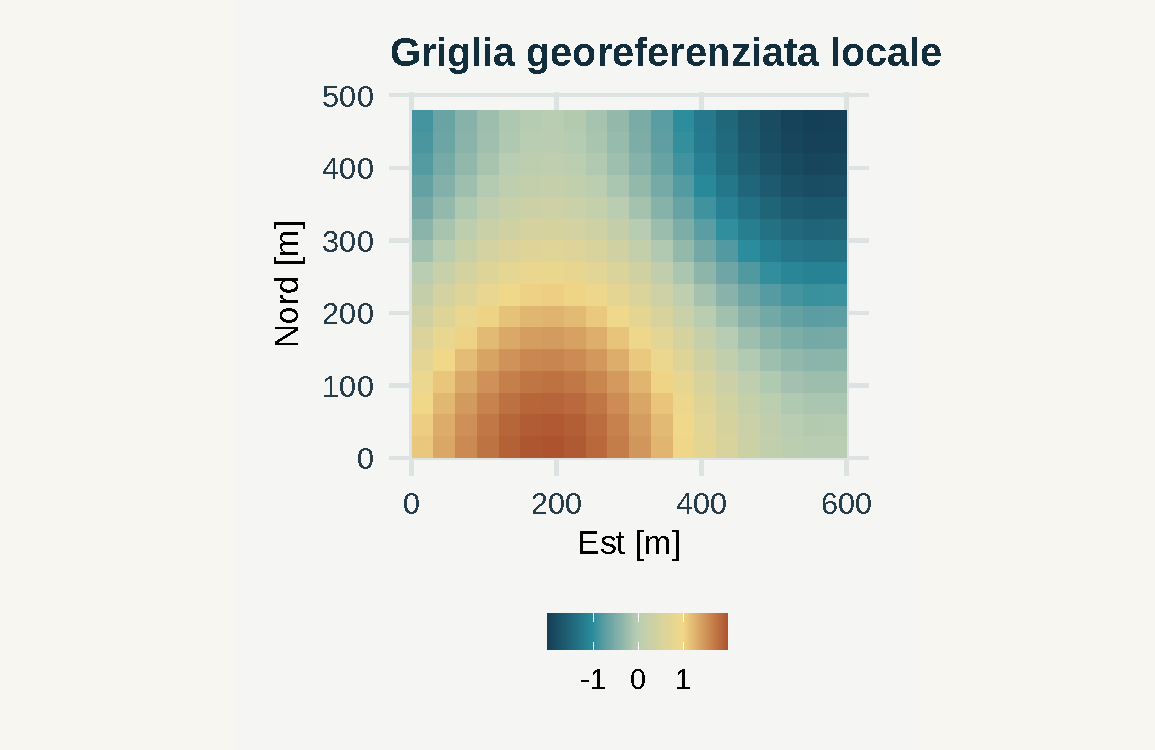
\includegraphics[width=\linewidth,height=6.0cm,keepaspectratio]{Esperimenti/m12-griglia-A.pdf}\par}
\PSmall{Lato della cella [m]: 30. Seme: 17.}
}};
\node[anchor=north west,inner sep=0] at([xshift=10.85cm,yshift=-2.12cm]current page.north west){\Colonna{8.16cm}{\PLabel{Scenario A · simulazione}
\PBody{La geometria di un raster collega righe e colonne a una superficie fisica. Nell’esperimento, il numero delle celle rimane costante mentre il controllo modifica il loro lato, espresso in metri. Le coordinate rappresentano i centri delle celle; superficie totale ed estensione verso Est vengono ricalcolate dalla risoluzione scelta.}
\par\smallskip{\centering\adjustbox{max width=.98\linewidth}{$\displaystyle A=n_rn_c\Delta x\Delta y$}\par\smallskip}
\PSmall{$n_{r}$ e $n_{c}$ indicano il numero di righe e colonne; Δx e Δy sono i lati della cella. A è la superficie totale, convertita da metri quadrati a ettari dividendo per diecimila.}
}};
\node[anchor=north east,inner sep=0] at([xshift=17.1cm,yshift=-12.04cm]current page.north west){\fontsize{7.7}{9}\selectfont \href{https://marzione00.github.io/Lab_Geo/\#laboratorio/m12-griglia}{\color{Classical}\bfseries Apri il laboratorio · m12-griglia}};
\end{tikzpicture}\end{frame}

\begin{frame}[plain]\hypertarget{slide21}{}
\bookmark[level=1,page=21]{Confronto | Geometria di una griglia raster}
\begin{tikzpicture}[remember picture,overlay]
\PilotChrome{Confronto | Geometria di una griglia raster}{LABORATORI DELLA SPEDIZIONE}{21}{La risoluzione e l’estensione del raster sono grandezze distinte.}
\node[anchor=north west,inner sep=0] at([xshift=.96cm,yshift=-2.12cm]current page.north west){\Colonna{9.40cm}{{\centering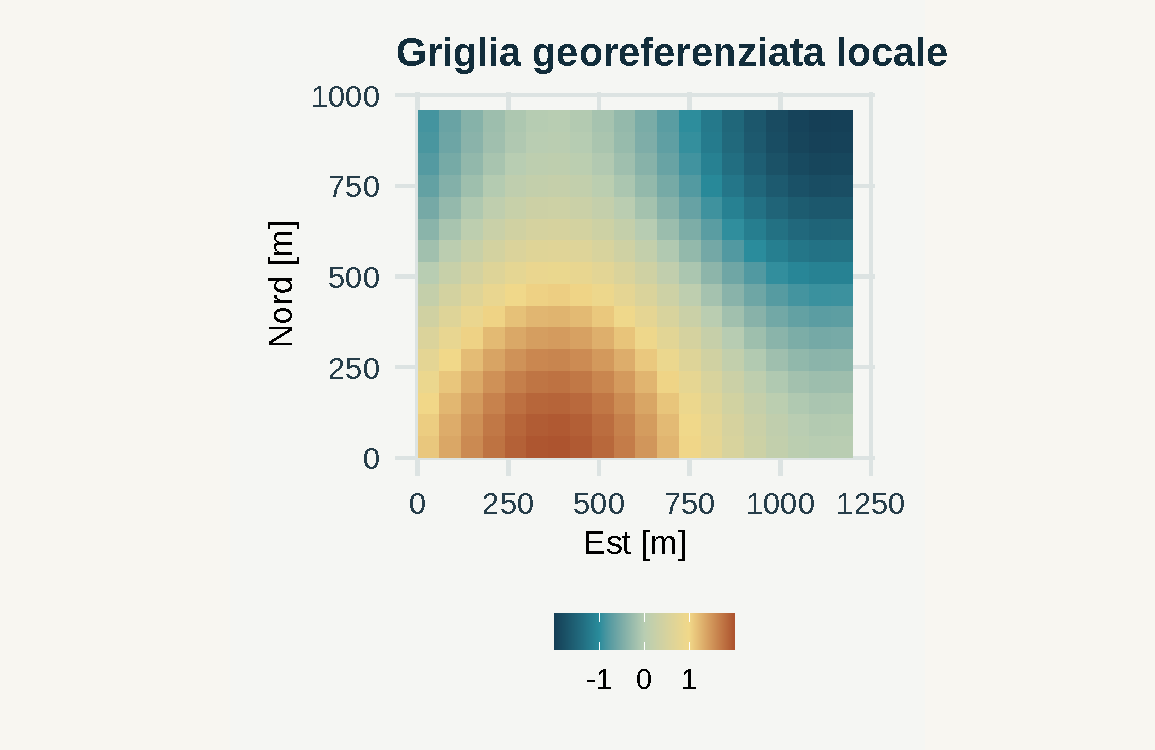
\includegraphics[width=\linewidth,height=5.6cm,keepaspectratio]{Esperimenti/m12-griglia-B.pdf}\par}
\PSmall{Lato della cella [m]: 30 $\to$ 60. Tutti gli altri parametri e il seme sono fissi.}
}};
\node[anchor=north west,inner sep=0] at([xshift=10.85cm,yshift=-2.12cm]current page.north west){\Colonna{8.16cm}{\PLabel{Confronto fra gli scenari}
{\fontsize{10.2}{12.8}\selectfont\begin{tabular}{@{}>{\raggedright\arraybackslash}p{0.48\linewidth}@{\hspace{.13cm}}>{\raggedright\arraybackslash}p{0.224\linewidth}@{\hspace{.13cm}}>{\raggedright\arraybackslash}p{0.224\linewidth}@{}}\toprule Grandezza & A & B\\[2.3pt]
\midrule 
Celle & 320 & 320\\[2.3pt]
Superficie [ha] & 28,8 & 115,2\\[2.3pt]
Estensione Est [m] & 600 & 1200\\[2.3pt]
\bottomrule\end{tabular}\par}
\vspace{.25cm}\PBody{Con celle di 60 metri il numero di celle resta 320, mentre la superficie passa da 28,8 a 115,2 ettari e l’estensione verso Est da 600 a 1200 metri. La risoluzione dichiarata determina ogni grandezza fisica ricavata dalla griglia.}
}};
\node[anchor=north east,inner sep=0] at([xshift=17.1cm,yshift=-12.04cm]current page.north west){\fontsize{7.7}{9}\selectfont \href{https://marzione00.github.io/Lab_Geo/\#laboratorio/m12-griglia}{\color{Classical}\bfseries Apri il laboratorio · m12-griglia}};
\end{tikzpicture}\end{frame}

\begin{frame}[plain]\hypertarget{slide22}{}
\bookmark[level=1,page=22]{Gradiente, pendenza ed esposizione}
\begin{tikzpicture}[remember picture,overlay]
\PilotChrome{Gradiente, pendenza ed esposizione}{LABORATORI DELLA SPEDIZIONE}{22}{Ricostruire derivate da differenze centrate e unità metriche.}
\node[anchor=north west,inner sep=0] at([xshift=.96cm,yshift=-2.12cm]current page.north west){\Colonna{9.40cm}{{\centering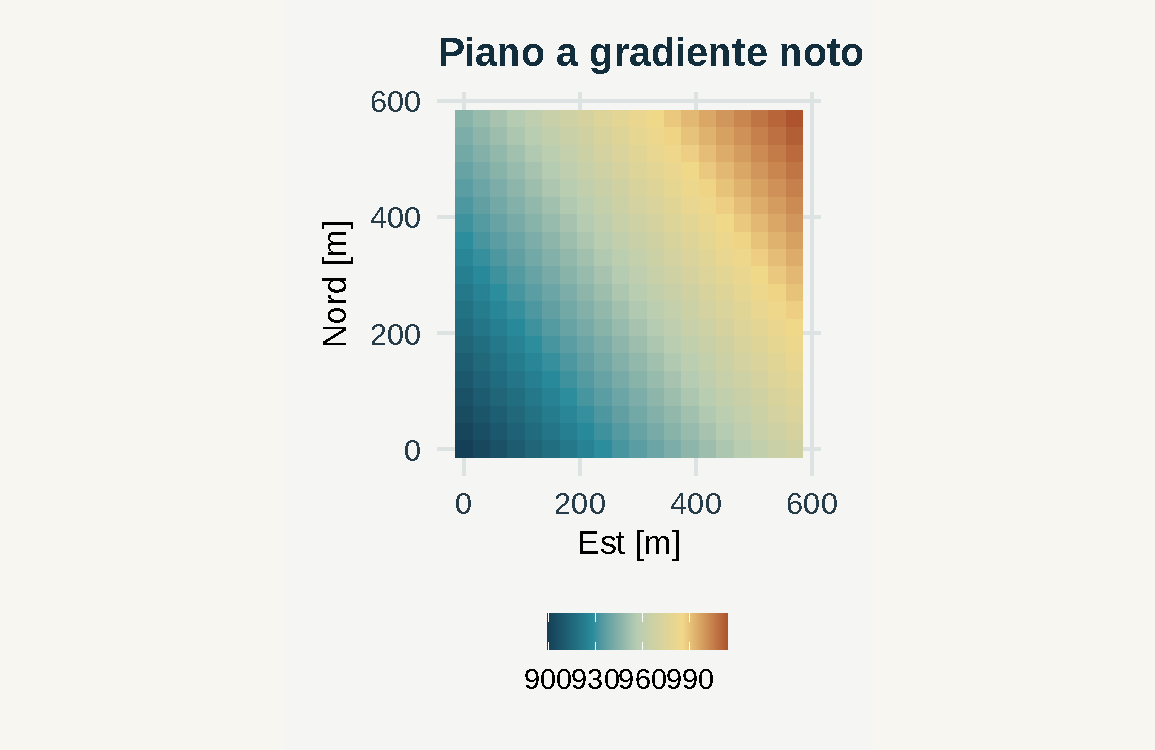
\includegraphics[width=\linewidth,height=5.0cm,keepaspectratio]{Esperimenti/m12-pendenza-A.pdf}\par}
\PSmall{Gradiente verso Est [m/m]: 0,12. Seme: 17.}
\PSmall{$g_{x}$ e $g_{y}$ sono le componenti del gradiente, Δx il passo metrico lungo Est e α l’angolo di pendenza. Nell’indicizzazione adottata dal codice, il primo indice della matrice varia lungo x; la percentuale è cento volte la norma del gradiente.}
}};
\node[anchor=north west,inner sep=0] at([xshift=10.85cm,yshift=-2.12cm]current page.north west){\Colonna{8.16cm}{\PLabel{Scenario A · simulazione}
\PBody{Un piano con gradienti noti permette di verificare la derivazione numerica prima di applicarla a un rilievo complesso. I controlli impostano l’aumento della quota per unità di distanza verso Est e verso Nord; il programma ricostruisce entrambe le derivate mediante differenze centrate, utilizzando quote e coordinate espresse in metri.}
\par\smallskip{\centering\adjustbox{max width=.98\linewidth}{$\displaystyle g_x=\frac{z_{i+1,j}-z_{i-1,j}}{2\Delta x},\quad\alpha=\arctan\sqrt{g_x^2+g_y^2}$}\par\smallskip}
}};
\node[anchor=north east,inner sep=0] at([xshift=17.1cm,yshift=-12.04cm]current page.north west){\fontsize{7.7}{9}\selectfont \href{https://marzione00.github.io/Lab_Geo/\#laboratorio/m12-pendenza}{\color{Classical}\bfseries Apri il laboratorio · m12-pendenza}};
\end{tikzpicture}\end{frame}

\begin{frame}[plain]\hypertarget{slide23}{}
\bookmark[level=1,page=23]{Confronto | Gradiente, pendenza ed esposizione}
\begin{tikzpicture}[remember picture,overlay]
\PilotChrome{Confronto | Gradiente, pendenza ed esposizione}{LABORATORI DELLA SPEDIZIONE}{23}{L’esposizione è definita dalla direzione di massima discesa; su un piano orizzontale rimane indeterminata.}
\node[anchor=north west,inner sep=0] at([xshift=.96cm,yshift=-2.12cm]current page.north west){\Colonna{9.40cm}{{\centering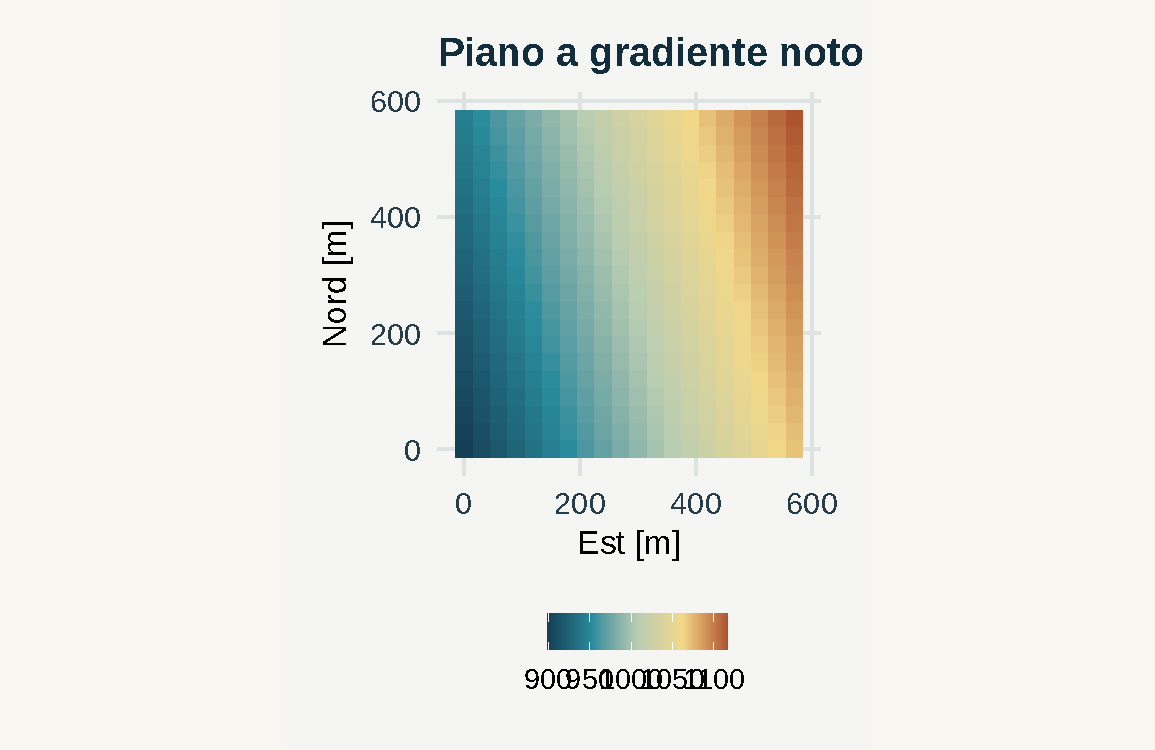
\includegraphics[width=\linewidth,height=5.6cm,keepaspectratio]{Esperimenti/m12-pendenza-B.pdf}\par}
\PSmall{Gradiente verso Est [m/m]: 0,12 $\to$ 0,3. Tutti gli altri parametri e il seme sono fissi.}
}};
\node[anchor=north west,inner sep=0] at([xshift=10.85cm,yshift=-2.12cm]current page.north west){\Colonna{8.16cm}{\PLabel{Confronto fra gli scenari}
{\fontsize{10.2}{12.8}\selectfont\begin{tabular}{@{}>{\raggedright\arraybackslash}p{0.48\linewidth}@{\hspace{.13cm}}>{\raggedright\arraybackslash}p{0.224\linewidth}@{\hspace{.13cm}}>{\raggedright\arraybackslash}p{0.224\linewidth}@{}}\toprule Grandezza & A & B\\[2.3pt]
\midrule 
Pendenza [gradi] & 8,21 & 17,2\\[2.3pt]
Pendenza [\%] & 14,4 & 31\\[2.3pt]
Esposizione [gradi da Nord] & 236 & 255\\[2.3pt]
Celle interne & 324 & 324\\[2.3pt]
\bottomrule\end{tabular}\par}
\vspace{.25cm}\PBody{Con gradiente verso Est di 0,3 la pendenza sale da 8,21 a 17,2 gradi, cioè da 14,4 a 31 per cento, e l’esposizione passa da 236 a 255 gradi da Nord. Angolo e percentuale derivano dalla stessa tangente.}
}};
\node[anchor=north east,inner sep=0] at([xshift=17.1cm,yshift=-12.04cm]current page.north west){\fontsize{7.7}{9}\selectfont \href{https://marzione00.github.io/Lab_Geo/\#laboratorio/m12-pendenza}{\color{Classical}\bfseries Apri il laboratorio · m12-pendenza}};
\end{tikzpicture}\end{frame}

\begin{frame}[plain]\hypertarget{slide24}{}
\bookmark[level=1,page=24]{Aggregazione e ricampionamento di una griglia}
\begin{tikzpicture}[remember picture,overlay]
\PilotChrome{Aggregazione e ricampionamento di una griglia}{LABORATORI DELLA SPEDIZIONE}{24}{Confrontare risoluzioni senza attribuire nuova informazione ai pixel interpolati.}
\node[anchor=north west,inner sep=0] at([xshift=.96cm,yshift=-2.12cm]current page.north west){\Colonna{9.40cm}{{\centering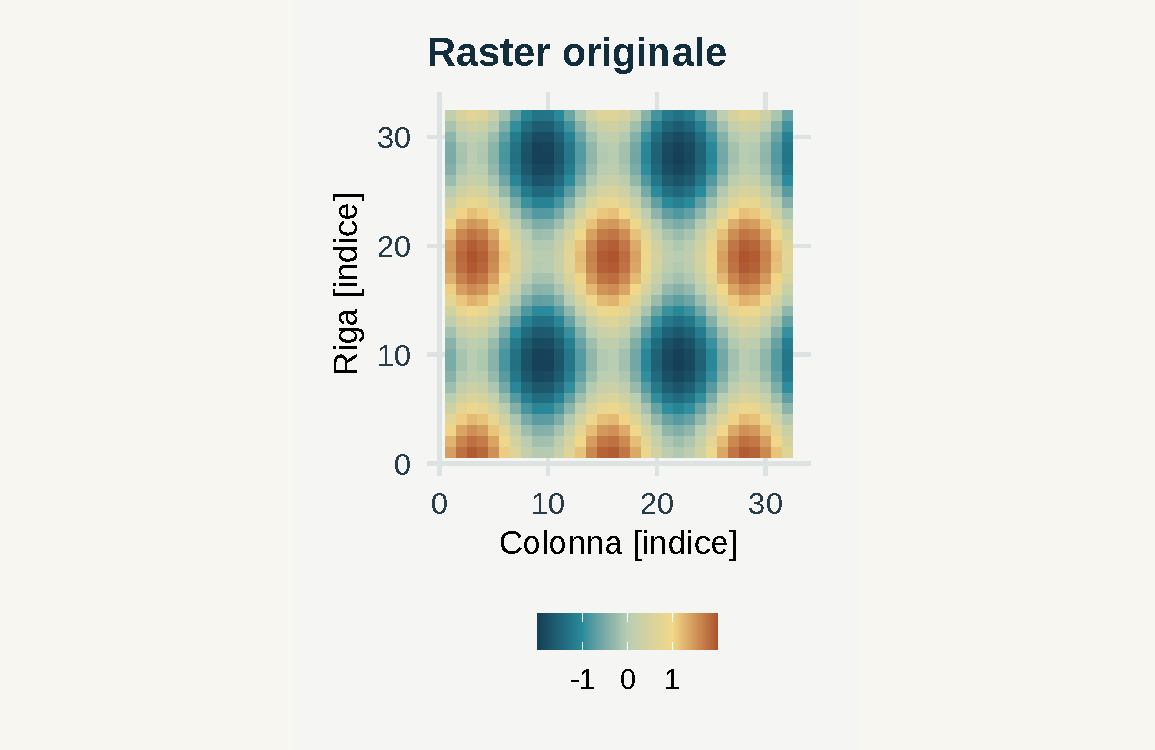
\includegraphics[width=\linewidth,height=5.0cm,keepaspectratio]{Esperimenti/m12-ricampionamento-A.pdf}\par}
\PSmall{Lato dei blocchi: 1 cella. Seme: 17.}
\PSmall{$\bar z_{celle}$ è la media dei valori originari e $\bar z_{blocchi}$ la media delle medie aggregate. L’uguaglianza mostrata presuppone blocchi completi con uguale numero di celle e uguale area.}
}};
\node[anchor=north west,inner sep=0] at([xshift=10.85cm,yshift=-2.12cm]current page.north west){\Colonna{8.16cm}{\PLabel{Scenario A · simulazione}
\PBody{L’aggregazione sostituisce gruppi di celle con una sintesi del loro contenuto. Nel raster dell’esperimento, i blocchi sono completi e hanno tutti la stessa dimensione, cosicché la media dei blocchi coincide con quella delle celle originarie. Cambiando il lato del blocco si riduce il numero dei valori memorizzati e si osserva quali strutture della superficie rimangano riconoscibili.}
\par\smallskip{\centering\adjustbox{max width=.98\linewidth}{$\displaystyle \bar z_{blocchi}=\bar z_{celle}\quad\text{per blocchi completi di uguale area}$}\par\smallskip}
}};
\node[anchor=north east,inner sep=0] at([xshift=17.1cm,yshift=-12.04cm]current page.north west){\fontsize{7.7}{9}\selectfont \href{https://marzione00.github.io/Lab_Geo/\#laboratorio/m12-ricampionamento}{\color{Classical}\bfseries Apri il laboratorio · m12-ricampionamento}};
\end{tikzpicture}\end{frame}

\begin{frame}[plain]\hypertarget{slide25}{}
\bookmark[level=1,page=25]{Confronto | Aggregazione e ricampionamento di una griglia}
\begin{tikzpicture}[remember picture,overlay]
\PilotChrome{{\fontsize{15.3}{19}\selectfont Confronto | Aggregazione e ricampionamento di una griglia}}{LABORATORI DELLA SPEDIZIONE}{25}{Con blocchi completi e celle di uguale area, la media delle medie conserva la media del raster.}
\node[anchor=north west,inner sep=0] at([xshift=.96cm,yshift=-2.12cm]current page.north west){\Colonna{9.40cm}{{\centering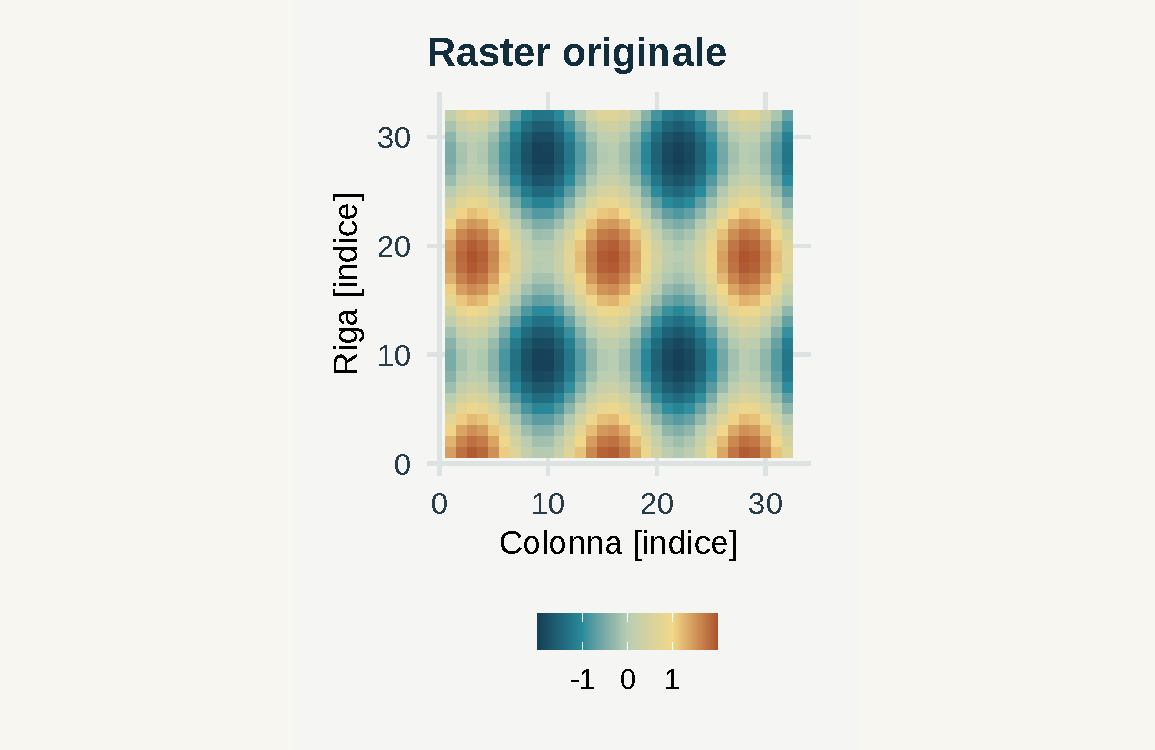
\includegraphics[width=\linewidth,height=5.6cm,keepaspectratio]{Esperimenti/m12-ricampionamento-B.pdf}\par}
\PSmall{Lato dei blocchi: 1 cella $\to$ 4 celle. Tutti gli altri parametri e il seme sono fissi.}
}};
\node[anchor=north west,inner sep=0] at([xshift=10.85cm,yshift=-2.12cm]current page.north west){\Colonna{8.16cm}{\PLabel{Confronto fra gli scenari}
{\fontsize{10.2}{12.8}\selectfont\begin{tabular}{@{}>{\raggedright\arraybackslash}p{0.48\linewidth}@{\hspace{.13cm}}>{\raggedright\arraybackslash}p{0.224\linewidth}@{\hspace{.13cm}}>{\raggedright\arraybackslash}p{0.224\linewidth}@{}}\toprule Grandezza & A & B\\[2.3pt]
\midrule 
Celle originali & 1024 & 1024\\[2.3pt]
Celle aggregate & 1024 & 64\\[2.3pt]
Scarto della media & 0 & $\approx 0$\\[2.3pt]
\bottomrule\end{tabular}\par}
\vspace{.25cm}\PBody{Con blocchi di quattro celle per lato le celle passano da 1024 a 64, e la media delle medie coincide con la media originale a meno di uno scarto dell’ordine di $10^{-18}$, dovuto all’aritmetica in virgola mobile. L’uguaglianza vale per blocchi completi di uguale area.}
}};
\node[anchor=north east,inner sep=0] at([xshift=17.1cm,yshift=-12.04cm]current page.north west){\fontsize{7.7}{9}\selectfont \href{https://marzione00.github.io/Lab_Geo/\#laboratorio/m12-ricampionamento}{\color{Classical}\bfseries Apri il laboratorio · m12-ricampionamento}};
\end{tikzpicture}\end{frame}

\begin{frame}[plain]\hypertarget{slide26}{}
\bookmark[level=1,page=26]{Dal risultato alla relazione}
\begin{tikzpicture}[remember picture,overlay]
\PilotChrome{Dal risultato alla relazione}{SINTESI}{26}{Riporta quote e pendenze con unità e denominatori, separando la descrizione della superficie dall’intervallo dei blocchi.}
\node[anchor=north west,inner sep=0] at([xshift=.96cm,yshift=-2.12cm]current page.north west){\Colonna{9.40cm}{\PLabel{Domanda di partenza}
\PBody{Quali quote e pendenze descrivono le due zone di un terreno sintetico, e che cosa misura un intervallo per la quota media?}
\PLabel{Risultato da discutere}
\PBody{La quota media è circa 1015,3 metri; la zona A, con 360 celle e 32,4 ettari, ha media 986,0 metri e la zona B 1044,6 metri. Le pendenze interne vanno da circa 0,49 a 28,5 gradi; il ricampionamento di dodici blocchi dà per la media un intervallo da 990,3 a 1039,0 metri.}
}};
\node[anchor=north west,inner sep=0] at([xshift=10.85cm,yshift=-2.12cm]current page.north west){\Colonna{8.16cm}{\PLabel{Limiti della conclusione}
\PBody{La superficie è sintetica e la sua georeferenziazione è fittizia. L’intervallo dei blocchi descrive la variabilità fra i dodici blocchi sotto la procedura adottata, mentre la media della superficie completa è già calcolabile esattamente.}
\vspace{.4cm}\href{https://marzione00.github.io/Lab_Geo/\#modulo-P08}{\color{Classical}\bfseries Prosegui · P08 · Collocare nel tempo il massimo di un proxy}
}};
\end{tikzpicture}\end{frame}

\begin{frame}[plain]\hypertarget{slide27}{}
\bookmark[level=1,page=27]{Fonti, dati e codice per riprodurre le figure}
\begin{tikzpicture}[remember picture,overlay]
\PilotChrome{Fonti, dati e codice per riprodurre le figure}{RIFERIMENTI}{27}{I risultati numerici si riferiscono ai dati e alle ipotesi dichiarate nel caso.}
\node[anchor=north west,inner sep=0] at([xshift=.96cm,yshift=-2.12cm]current page.north west){\Colonna{9.40cm}{\PLabel{Dati e attribuzioni}
\PBody{Raster sintetico del corso (raster\_v3.csv e raster\_v3.tif) con sistema di riferimento fittizio; lettura e derivate secondo la documentazione del pacchetto terra, in raccordo con il modulo M12.}
}};
\node[anchor=north west,inner sep=0] at([xshift=10.85cm,yshift=-2.12cm]current page.north west){\Colonna{8.16cm}{\PLabel{Nell’archivio dei sorgenti}
\PBody{Codice contiene i frammenti delle pagine; R contiene lo script P07\_figure.R, che ricostruisce figure e valori dai dati. Esperimenti comprende i programmi dei due scenari, Diagrammi i disegni TikZ modificabili, Scena il modello Blender della copertina.}
\vspace{.4cm}\href{https://marzione00.github.io/Lab_Geo/\#modulo-P07}{\color{Classical}\bfseries Apri la spedizione P07 su GeoStat Lab}
}};
\end{tikzpicture}\end{frame}
\end{document}
